% ============================================================================
%  SoLD -- one-page-per-section summary of Results and Discussion
%  Standalone document. Compile on its own; it reuses the figures already in
%  fig/main and fig/supp, so keep it in the same Overleaf project root as
%  main.tex. No other new files are needed.
% ============================================================================
\documentclass[11pt]{article}

\usepackage[margin=2.2cm]{geometry}
\usepackage{graphicx}
\usepackage{enumitem}
\usepackage{xcolor}
\usepackage[hidelinks]{hyperref}
\usepackage{titlesec}
\usepackage{parskip}
\usepackage{caption}
\usepackage{float}

\definecolor{accent}{HTML}{2C5F7C}
\titleformat{\section}{\Large\bfseries\color{accent}}{\thesection.}{0.5em}{}
\titleformat{\subsection}{\normalsize\bfseries}{\thesubsection}{0.5em}{}
\setlist[itemize]{leftmargin=1.2em, itemsep=1pt, topsep=3pt, parsep=0pt}
\captionsetup{font=small, labelfont=bf, labelformat=empty}
\newcommand{\lead}[1]{\textbf{#1}}
\setcounter{secnumdepth}{2}

\begin{document}

\begin{center}
{\LARGE\bfseries The Sorghum Lipid Database (SoLD)}\\[2pt]
{\large Summary of Results and Discussion}\\[6pt]
\end{center}

\noindent\textbf{Design.} The Sorghum Association Panel grown in two field
trials. \textbf{CTL} is 2019, nutrient-sufficient, standard planting date.
\textbf{LIN} is 2022, reduced nitrogen and phosphorus, earlier planting to
impose cold at establishment, and no insecticide, herbicide or pesticide.
394 accessions in CTL and 363 in LIN; 243 lipid species quantified by
high-resolution LC--MS.

\vspace{4pt}
\hrule
\vspace{6pt}

\section{Results}

\subsection{QC and normalization}
\begin{itemize}
  \item \lead{Method.} SERRF normalization on the vendor peak tables, then
        SpATS spatial correction for field position, with model residuals added
        back to the fitted mean so genotype signal is preserved. QC-RSD compared
        before and after SERRF, plus run-order drift, injection-level PCA, and
        maps of SpATS residuals across the field.
  \item \lead{Found.} Analytical performance is comparable between trials, so
        CTL--LIN differences downstream are not instrument drift. Spatial
        correction removes plot-to-plot field variation that would otherwise
        look like genotype effects.
\end{itemize}

\begin{figure}[H]
\centering
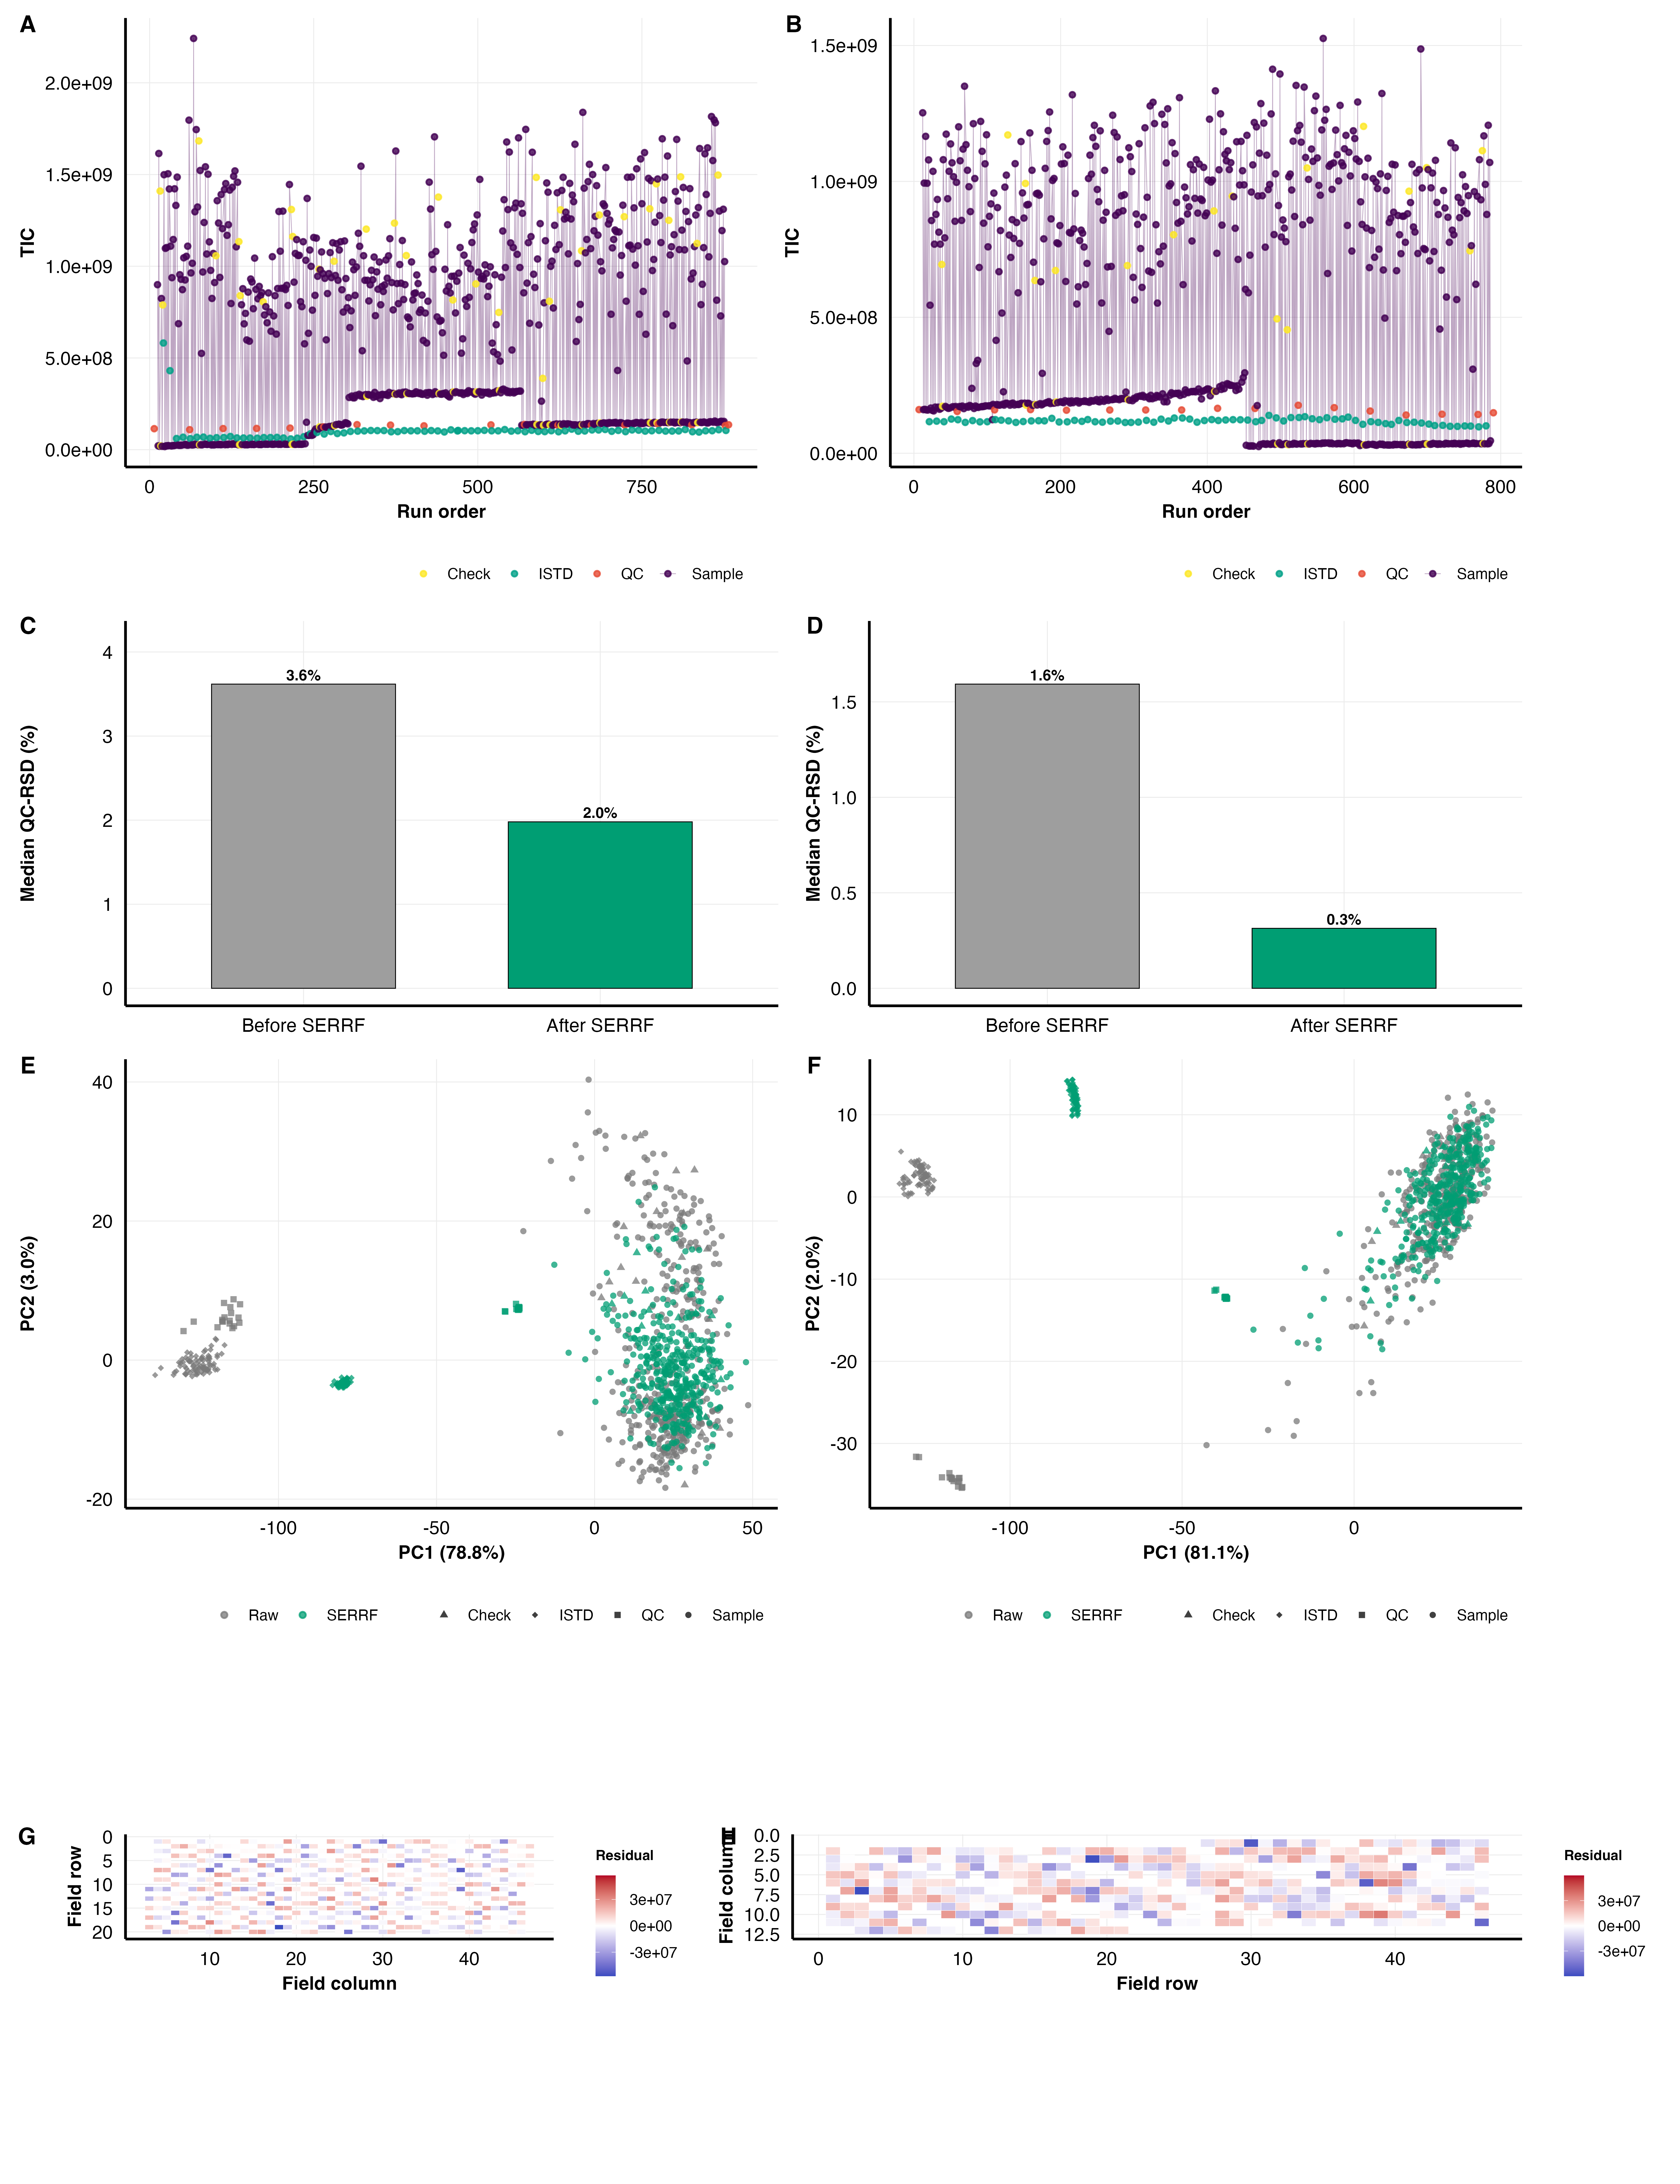
\includegraphics[width=0.86\textwidth]{fig/supp/SuppFig_S2_QC_RunOrder_SERRF_PCA_SpATS.png}
\caption{Supp.\ Fig.\ S2. QC diagnostics -- run order, SERRF normalization,
injection PCA, and SpATS spatial correction.}
\end{figure}

\subsection{Race and population structure explain almost nothing}
\begin{itemize}
  \item \lead{Method.} Kruskal--Wallis with
        $\varepsilon^2 = (H-k+1)/(n-k)$ as effect size, truncated at zero and
        BH-corrected. Two groupings tested -- the five classical botanical races
        plus a Mixed group, and six marker-based genetic clusters. Plus a PCA of
        the 13-class composition per trial on log$_{10}$ values scaled to unit
        variance.
  \item \lead{Race explains nothing.} No trait significant in either trial after
        BH correction (smallest $q=0.468$; effects $\varepsilon^2 \leq 0.027$).
  \item \lead{Genetic cluster explains one thing.} PS under LIN
        ($q=1.11\times10^{-6}$, $\varepsilon^2=0.104$). Under CTL the same trait
        gives only a weak, non-significant trend.
  \item \lead{Ordination agrees.} Accessions of one race or cluster are dispersed
        rather than grouped; race or cluster explains at most 1.6\% of variance.
  \item \lead{Why it matters.} The lipidome is not a readout of population
        history, so lipid GWAS in this panel is not re-discovering structure.
\end{itemize}

\begin{figure}[H]
\centering
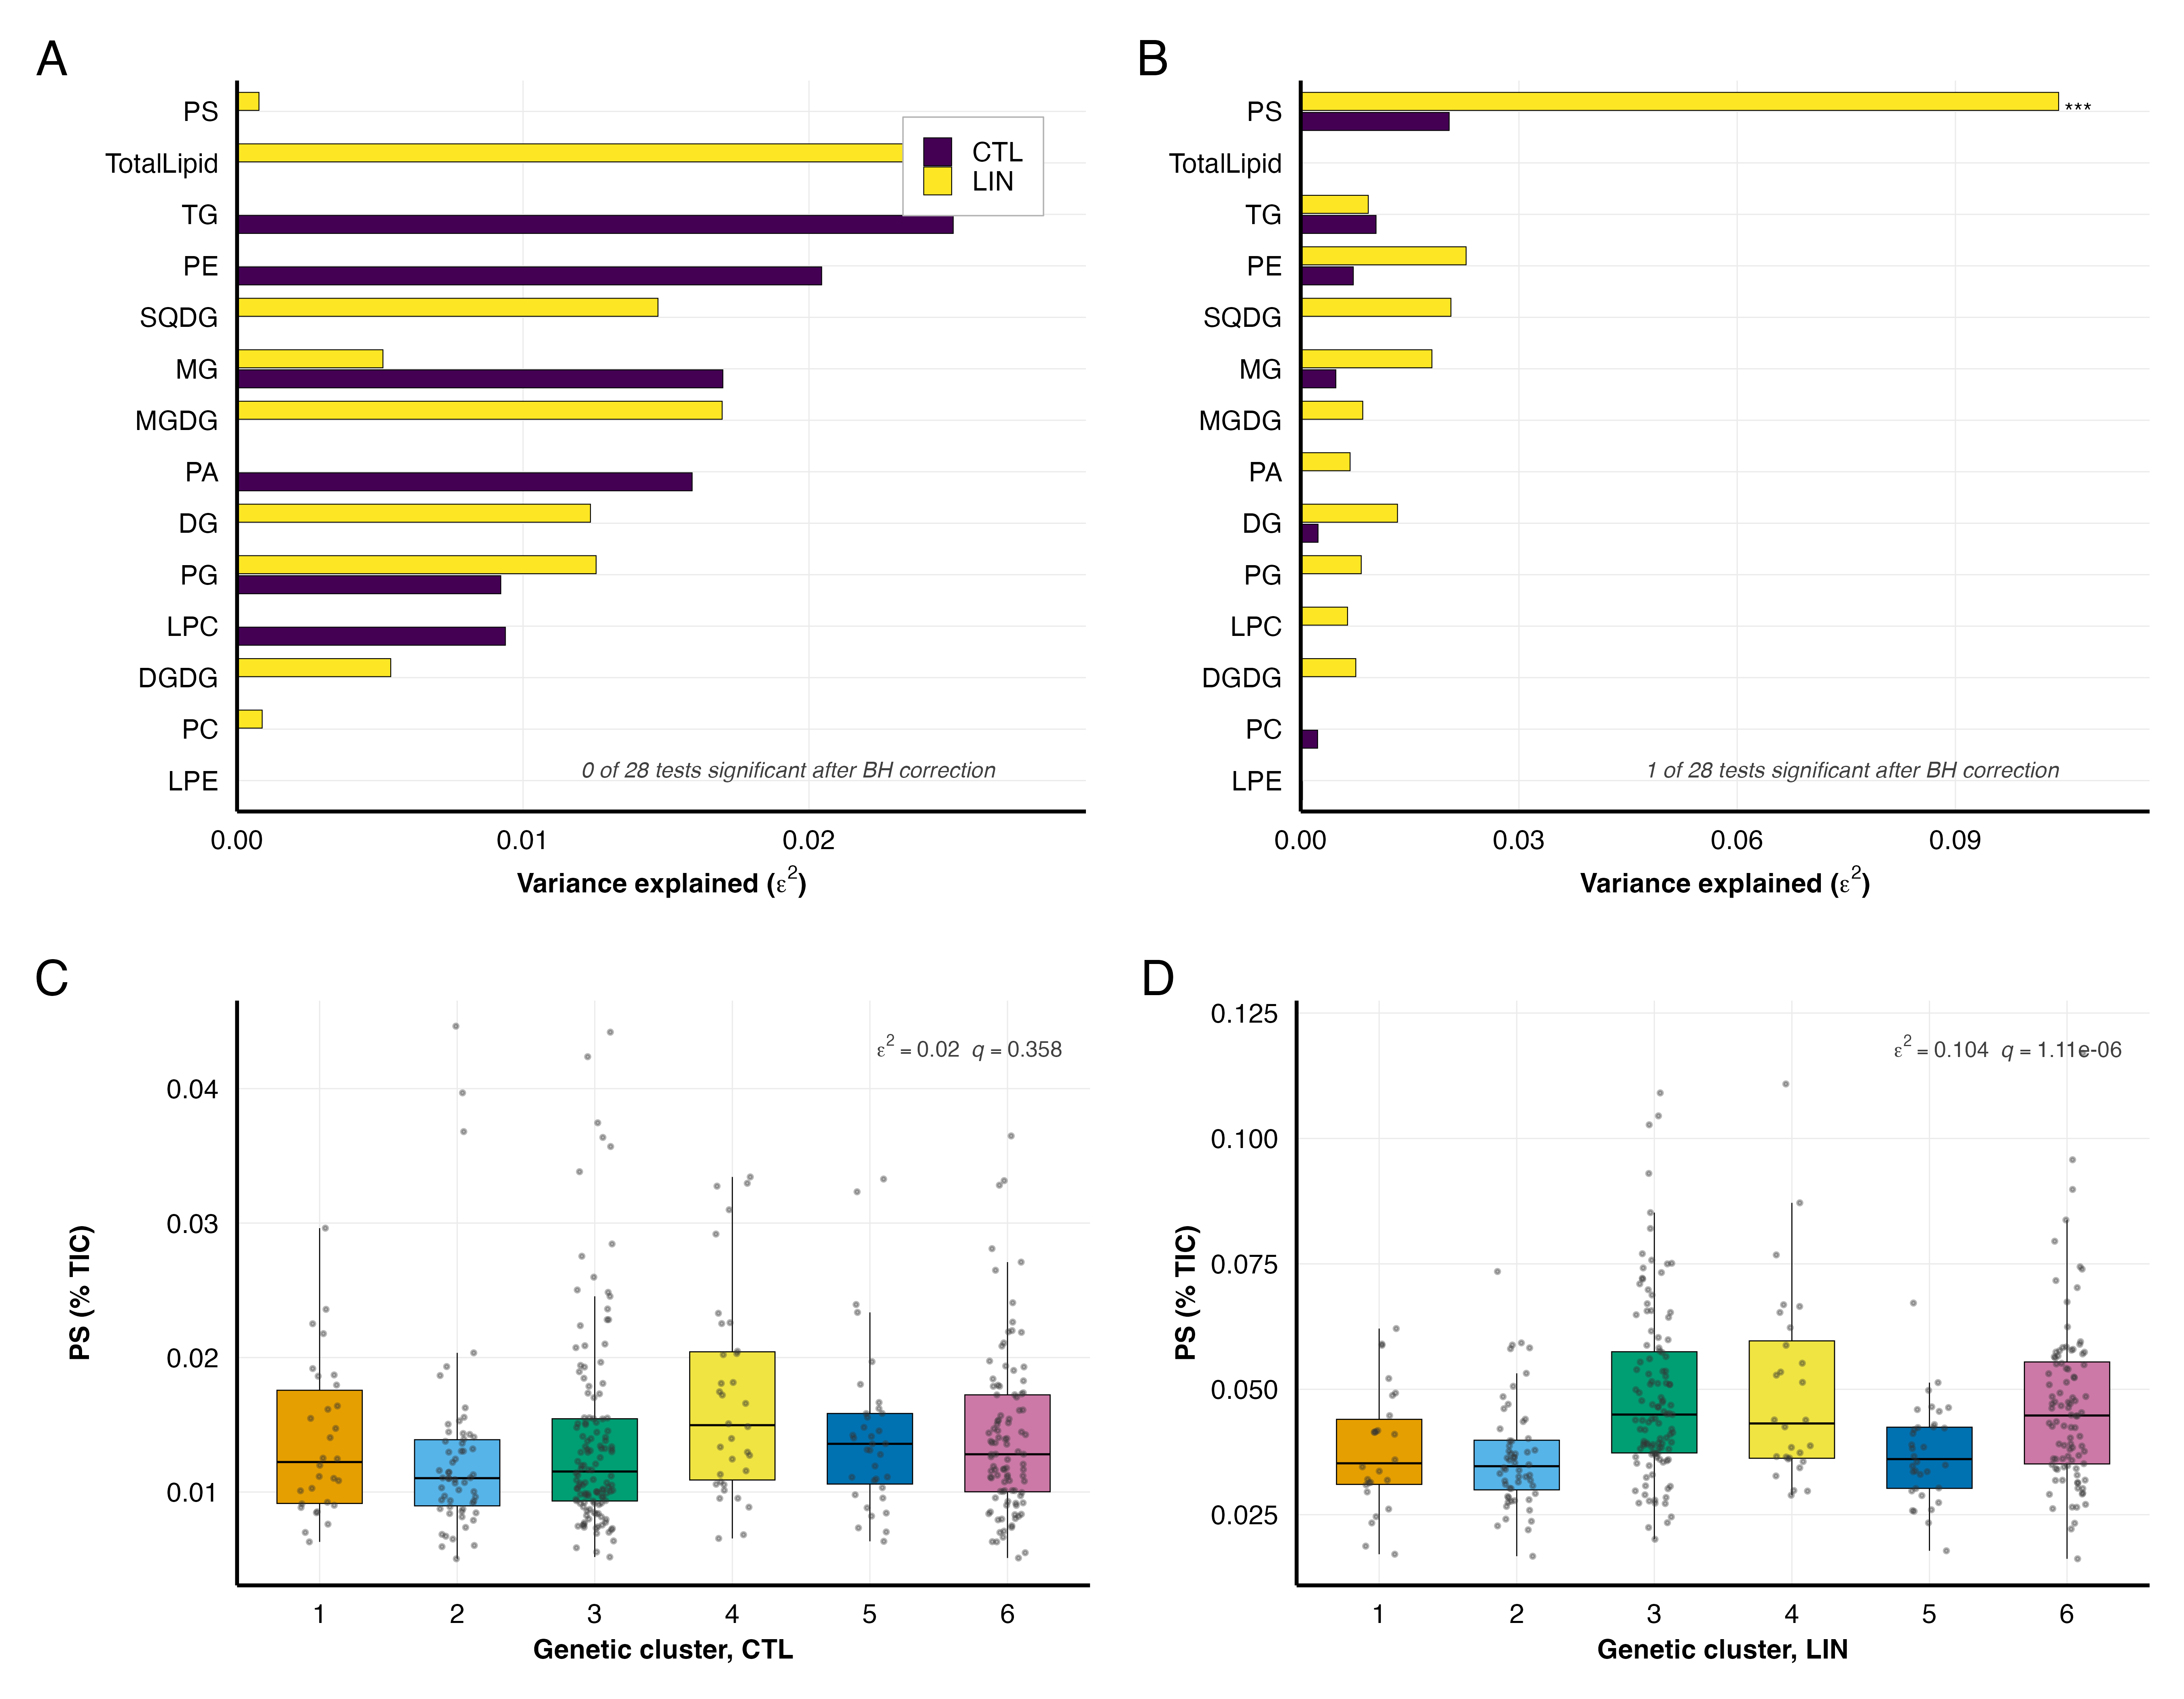
\includegraphics[width=0.9\textwidth]{fig/main/Figure1_Population_Structure.png}
\caption{Figure 1. Botanical race and marker-based cluster explain little
lipid-class variation; PS under LIN is the single exception.}
\end{figure}

\clearpage
\subsection{Lipidome overview and the four compositional axes}
\begin{itemize}
  \item \lead{Method.} Species inventory; composition as \%TIC taken per sample
        and then averaged, so a few high-signal samples cannot dominate;
        species-level PCA within each trial; LION ontology enrichment as the one
        direct CTL--LIN contrast.
  \item \lead{Inventory.} 243 species -- 152 in both trials, 49 CTL-only, 42
        LIN-only, where trial-specific means below detection threshold rather
        than confirmed absent.
  \item \lead{Composition.} MGDG 32.3 $\rightarrow$ 29.8\%, PC 24.0 $\rightarrow$
        23.1\%, DGDG 12.0 $\rightarrow$ 12.1\%, DG 12.9 $\rightarrow$ 13.8\%,
        \textbf{TG 2.6 $\rightarrow$ 5.0\%}, \textbf{SQDG 2.7 $\rightarrow$
        1.3\%}. The 13 focal classes are $\approx$93\% of annotated signal.
  \item \lead{Minor pools.} Sterols show the largest \emph{proportional} change of
        any superclass, 0.042 $\rightarrow$ 0.215\%, almost all
        $\beta$-sitosterol at 4.6-fold.
  \item \lead{Structure.} Lipid class strongly structures species-level variation;
        TG forms a distinct cluster away from membrane lipids in both trials.
  \item \lead{LION.} A head-group charge contrast, with storage and lipid-droplet
        terms up under LIN and glycerophospholipid and membrane-component terms
        down.
  \item \lead{The four axes, defined here.} (i)~low SQDG, (ii)~high TG,
        (iii)~a PS-centred phospholipid shift, (iv)~an LPC/LPE balance shifted
        toward LPE (LPC flat, LPE up 1.4-fold, ratio 17.0 $\rightarrow$ 11.3).
\end{itemize}

\begin{figure}[H]
\centering
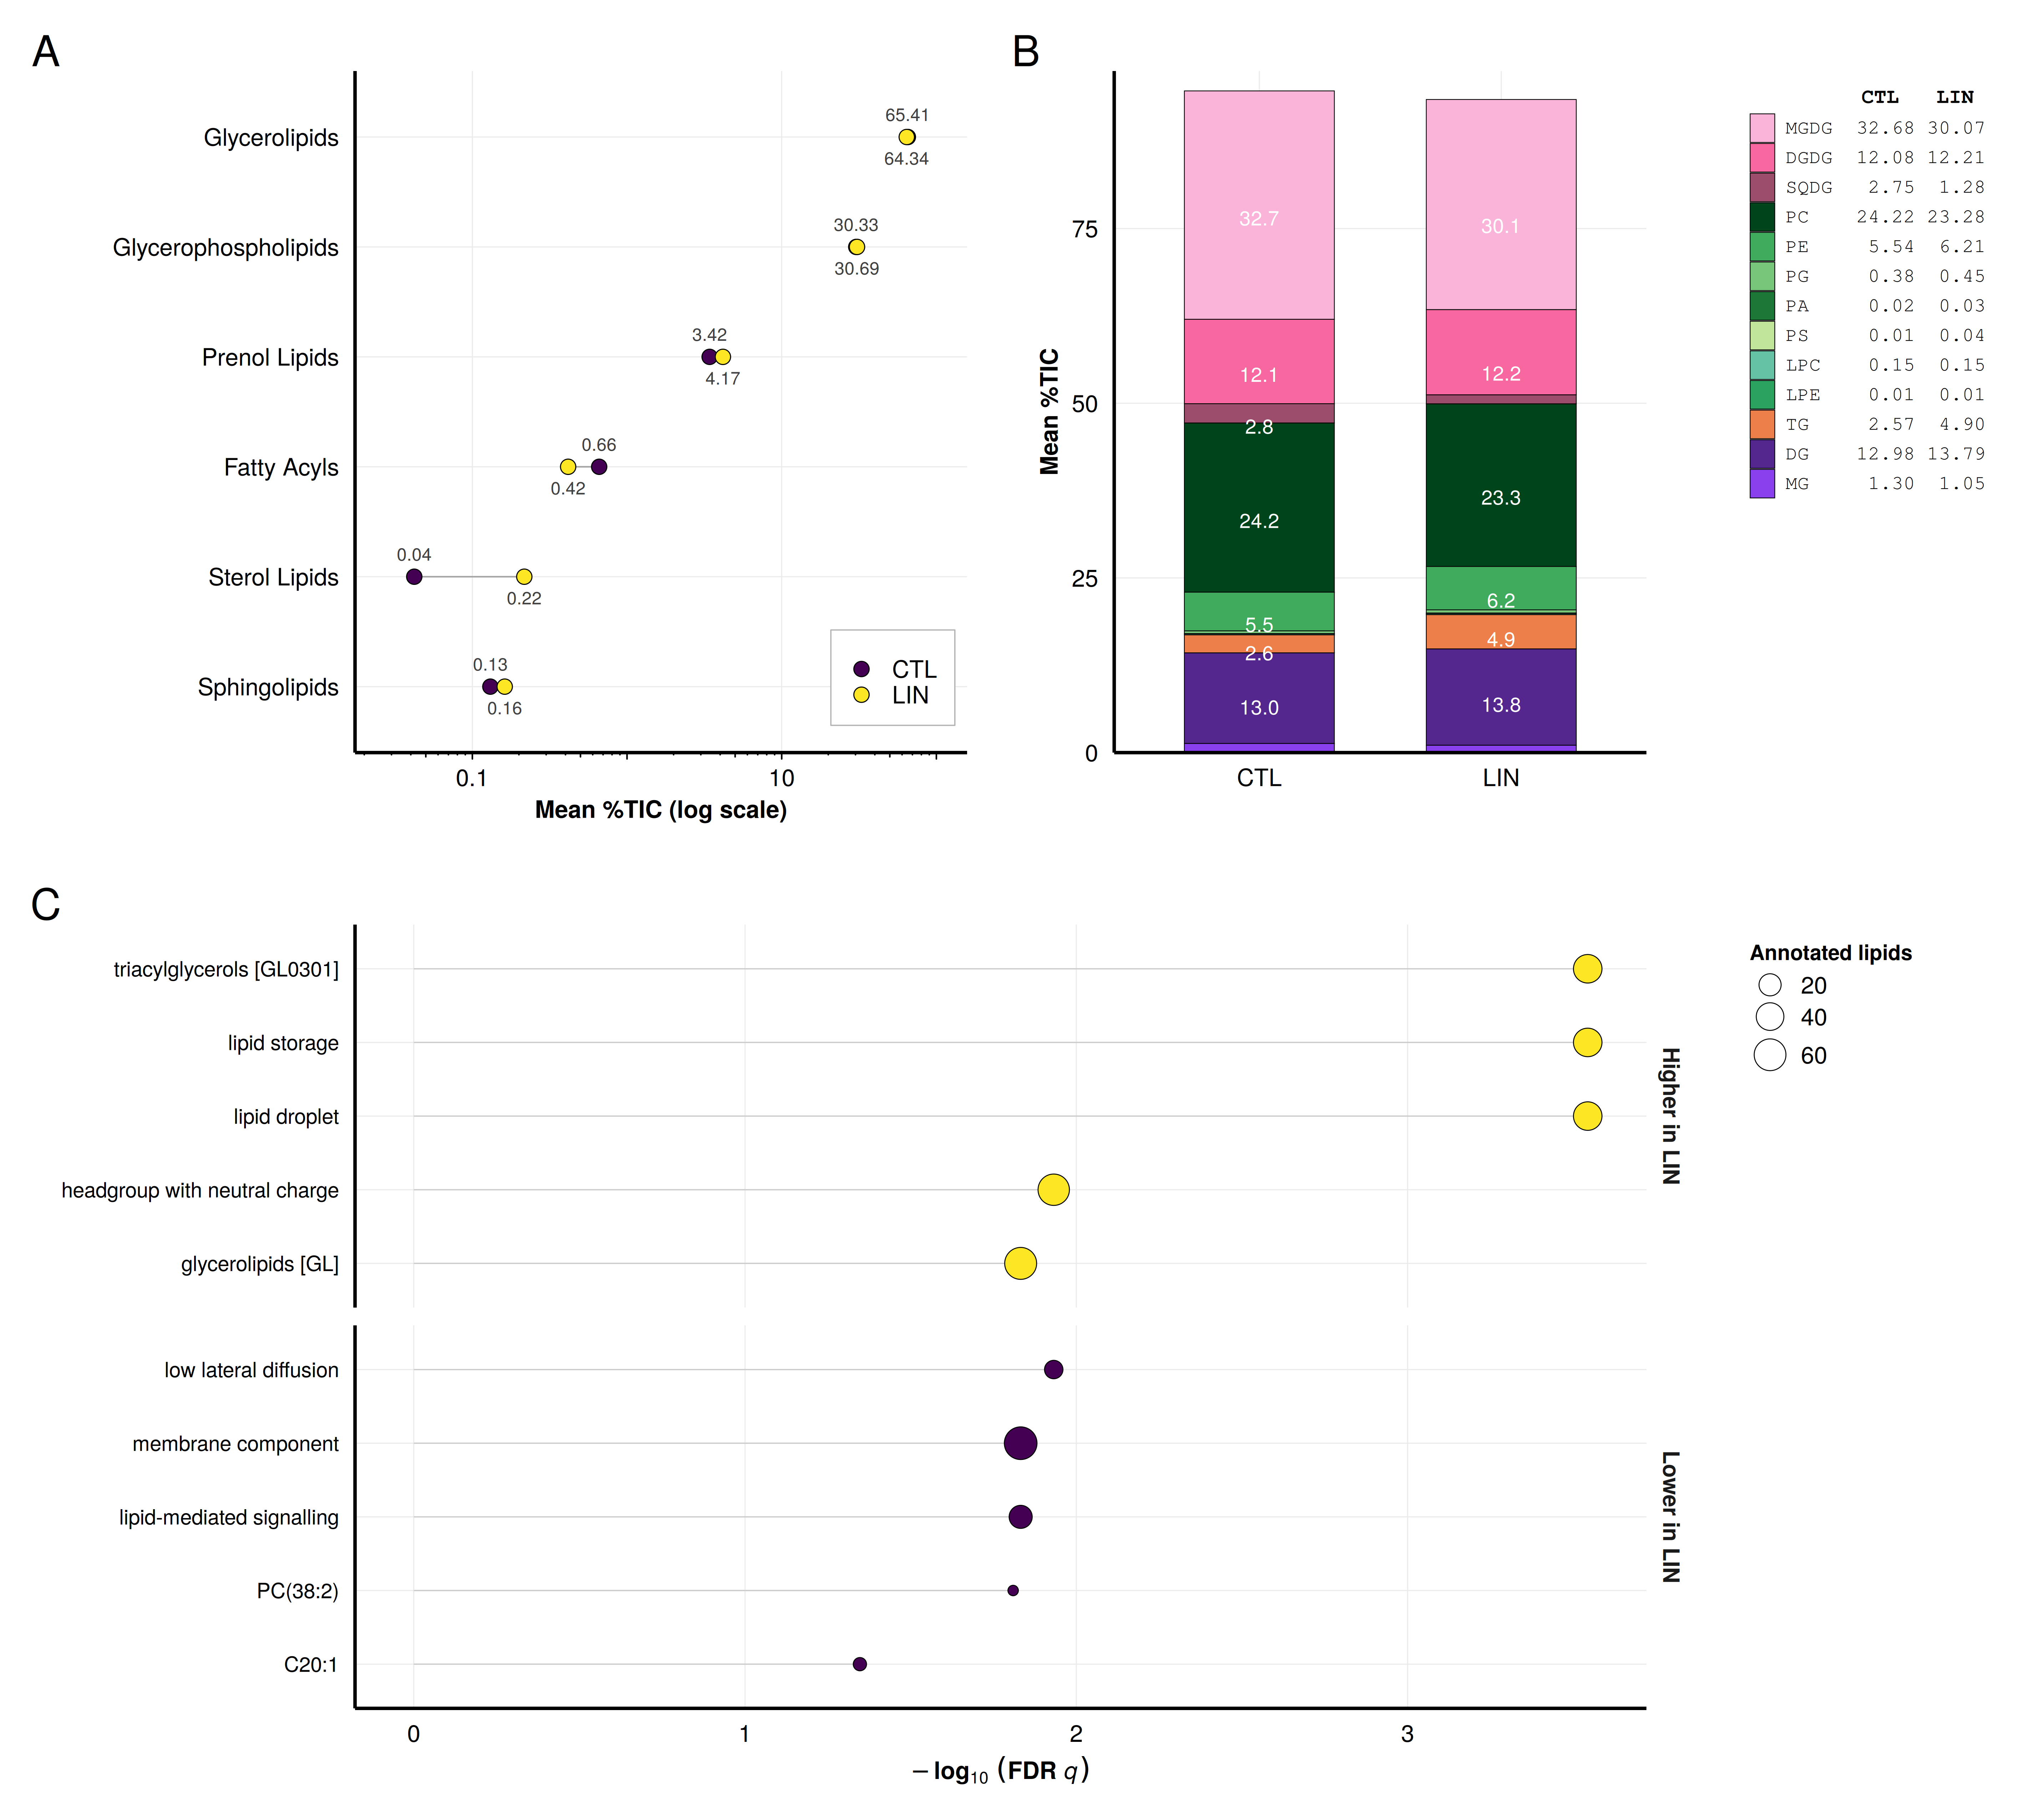
\includegraphics[width=0.95\textwidth]{fig/main/Figure2_Class_Composition.png}
\caption{Figure 2. Lipid-class composition. (A)~every annotated superclass on a
log scale; (B)~the 13 focal classes; (C)~LION ontology terms, the only direct
CTL--LIN contrast in the figure.}
\end{figure}

\clearpage
\subsection{GWAS}
\begin{itemize}
  \item \lead{Method.} GEMMA univariate mixed linear model, centered kinship from
        SNP genotypes, first three genotype PCs as covariates, MAF 0.05 and
        heterozygosity 0.8 filters, Bonferroni threshold
        $p \leq 8.19\times10^{-9}$. Run for every individual species, every class
        sum and every class ratio, in both trials.
  \item \lead{Found.} Association signal is concentrated under CTL and diffuse
        under LIN -- fewer, sharper peaks in the control trial against a broader,
        more distributed architecture in low-input.
\end{itemize}

\begin{figure}[H]
\centering
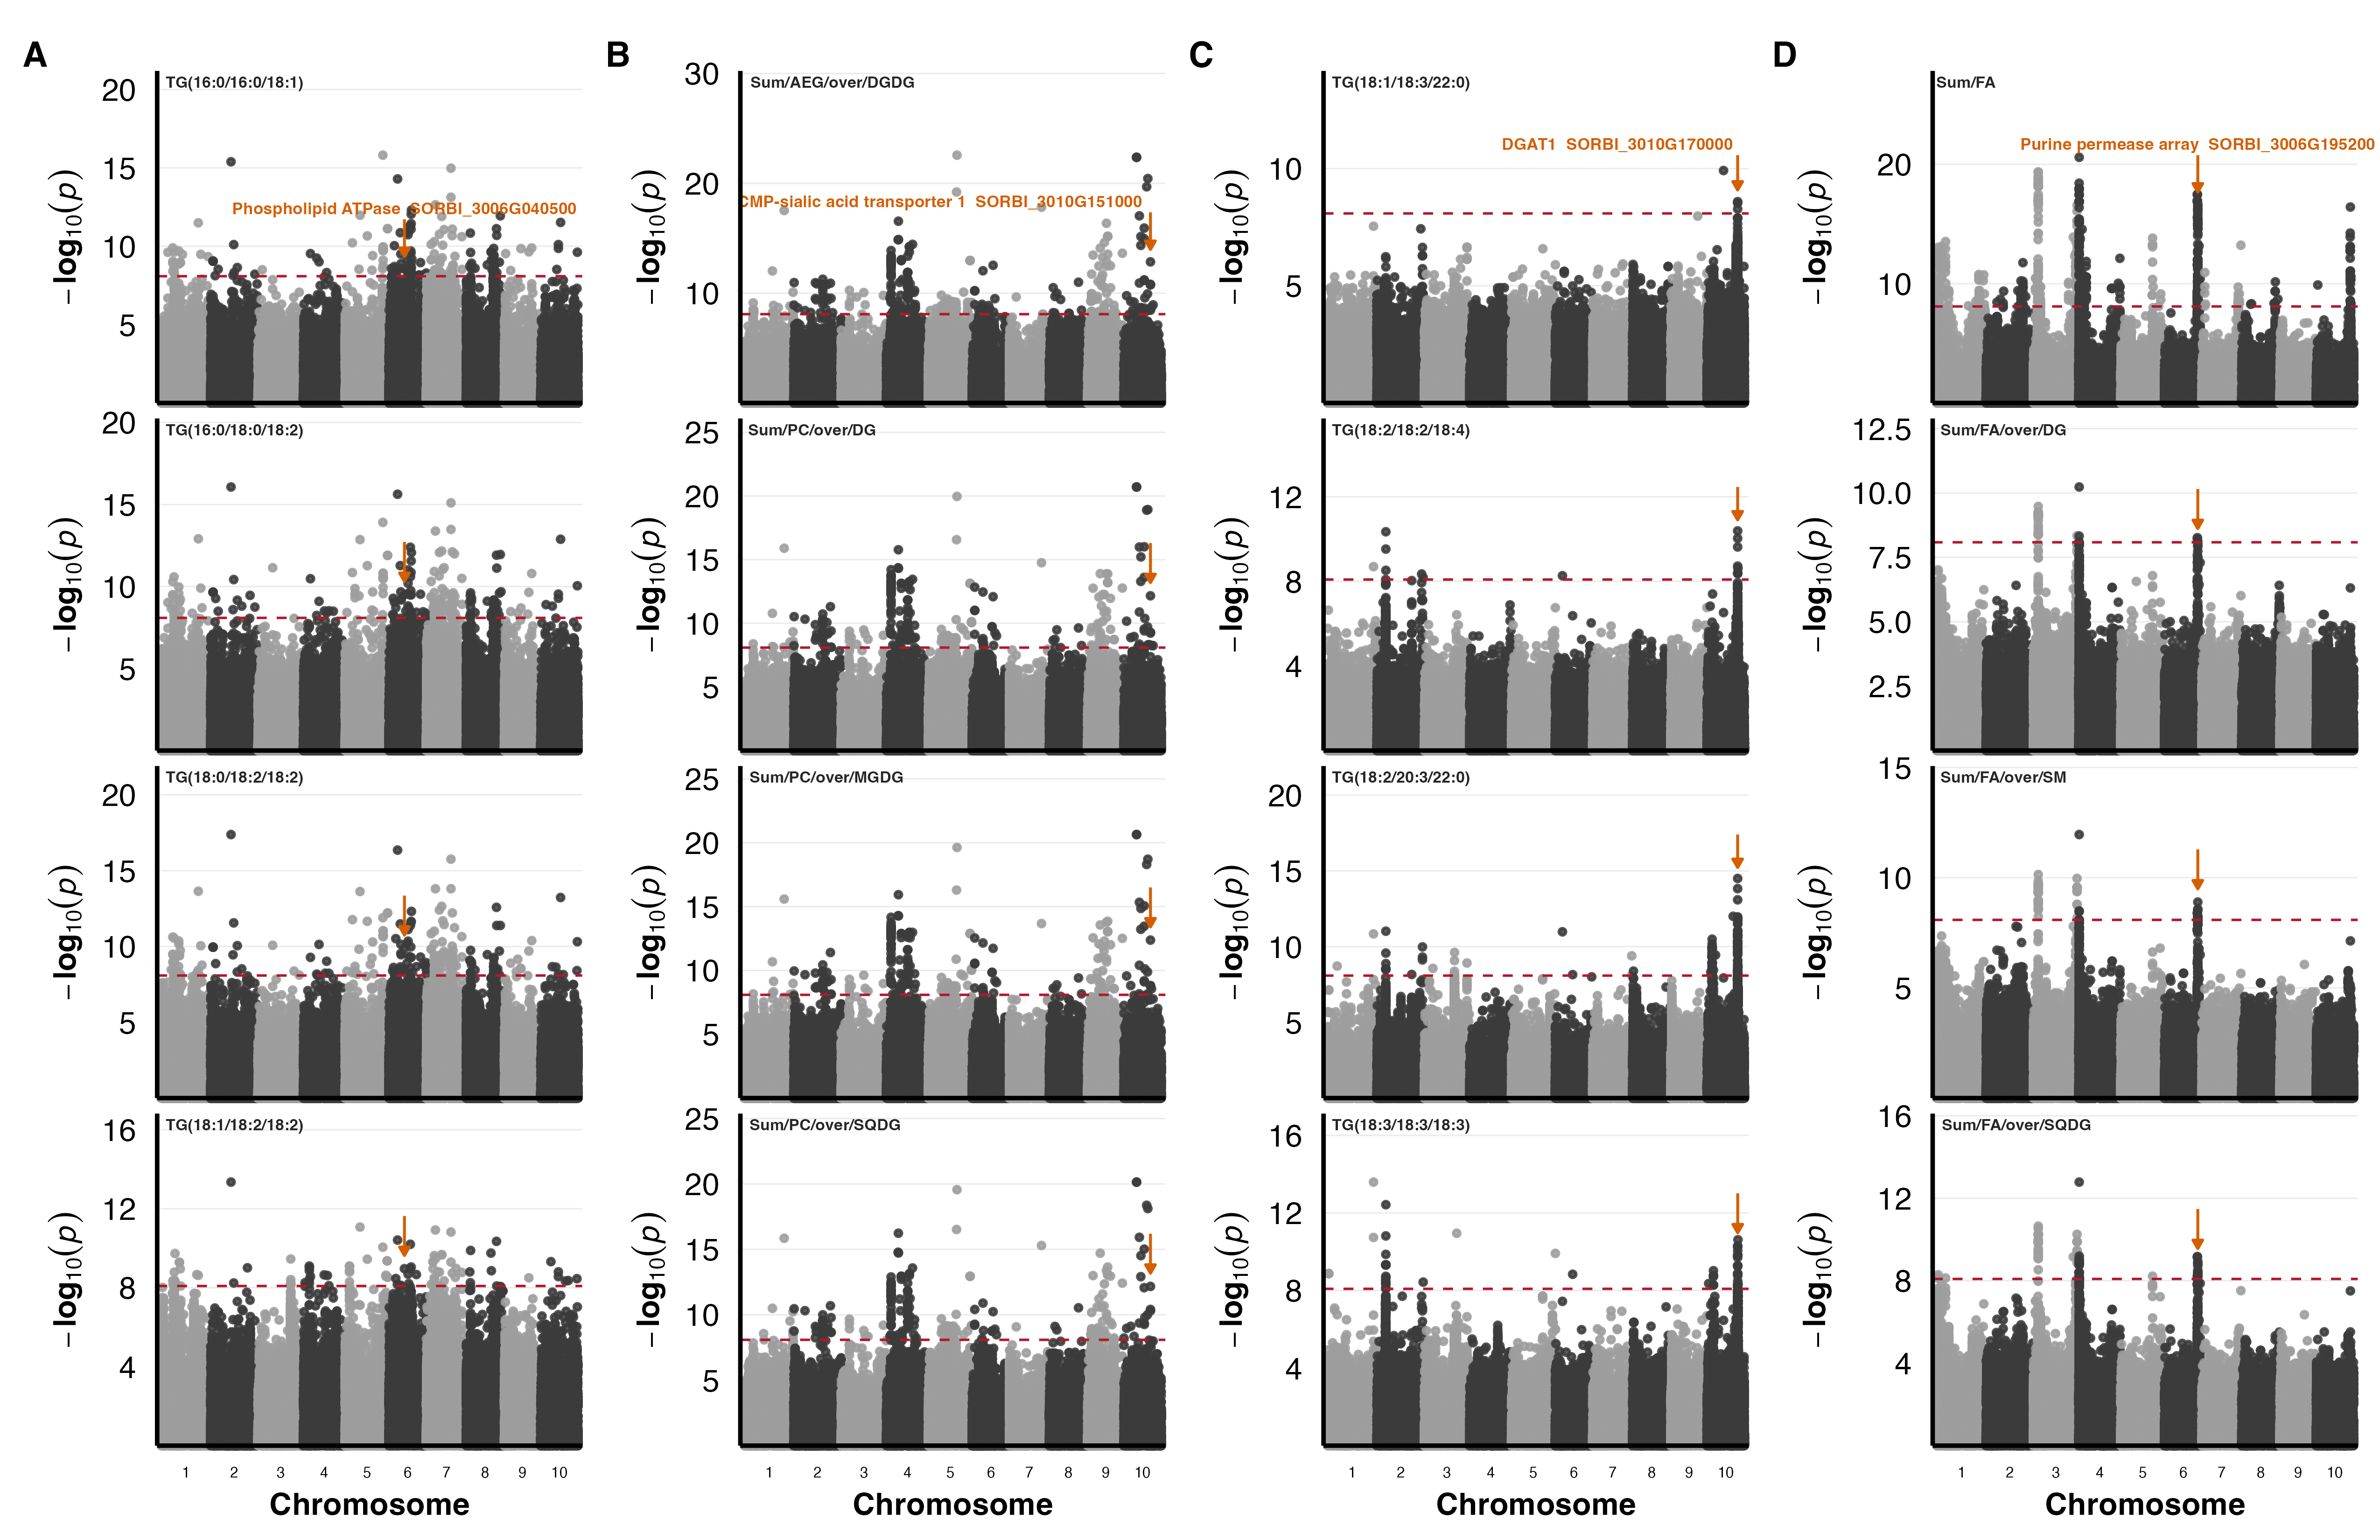
\includegraphics[width=0.92\textwidth]{fig/main/Figure3_GWAS_Manhattan.png}
\caption{Figure 3. Manhattan plots for representative traits in each trial and
trait layer. Arrows mark the candidate loci discussed in the text.}
\end{figure}

\subsection{GO enrichment -- the principal methods contribution}

\noindent This is the part worth reading in full. Four steps:

\begin{enumerate}[leftmargin=1.4em, itemsep=3pt]
  \item \lead{Stratified testing.} GO over-representation is run \emph{separately}
        within each lipid class $\times$ trial $\times$ trait layer $\times$
        ontology. Stratifying by class is what makes a term interpretable, since
        it attributes an enrichment to the traits of one class rather than to the
        candidate set as a whole.
  \item \lead{LD-aware permutation null.} In sorghum a significant SNP tags every
        gene in its LD window rather than one gene, so a naive GO test counts the
        same association repeatedly and inflates significance. Every term was
        therefore tested against a null built from 8{,}000 random draws of
        \textbf{gene-density-matched 250~kb intervals}. Density matching matters
        because gene-dense regions contribute more genes and would otherwise
        appear enriched for everything. This yields $q_{\mathrm{LD}}$, corrected
        for mapping structure rather than only for multiple testing.
  \item \lead{Two-pass collapse.} Two things inflate the term list. The Gene
        Ontology nests parent and child terms, so one gene set surfaces as several
        terms; and class sums and ratios share candidate genes by construction, so
        one gene set recurs across classes, layers and both ontologies. Terms with
        \emph{identical} candidate-gene sets were merged, first within a stratum
        and then across strata.
  \item \lead{Interpretability filter.} For the main figure, only loci whose GO
        term draws on at most 30 background genes. This is a criterion of
        specificity, not of significance -- \emph{zinc ion binding}
        (1{,}015 background genes) passes the permutation null while naming no
        biological process. Interval count was deliberately \emph{not} used to
        select terms, because it scales with GO term size and would discriminate
        against precisely the small, specific terms of interest (terms in three or
        more intervals average 175 background genes at 10-fold enrichment; those
        below average 24 genes at 23-fold).
\end{enumerate}

\begin{itemize}
  \item \lead{Numbers.} 103 enrichments $\rightarrow$ 101 pass the LD-aware null
        $\rightarrow$ collapse to \textbf{50 distinct loci} (17 CTL, 33 LIN)
        $\rightarrow$ 19 shown in Figure 4.
  \item \lead{The asymmetry is real, not a filter artefact.} 17 CTL loci against
        33 LIN, from roughly half as many candidate genes, and all but one CTL
        survivor is a broad category.
  \item \lead{LIN names processes.} Nitrate assimilation and transport 31-fold,
        cellular response to phosphate starvation 17.4-fold, sphingolipid
        metabolic process 32.5-fold, jasmonate signalling / defense / wounding
        34.5-fold.
  \item \lead{CTL does not.} Zinc ion binding, proteolysis, peptidase activity,
        transmembrane transport.
  \item \lead{Two failure modes illustrated.} The purine permeases are specific but
        reduce to one tandem array recovered 25 times; zinc ion binding is spread
        over six to eight intervals but names nothing.
\end{itemize}

\begin{figure}[H]
\centering
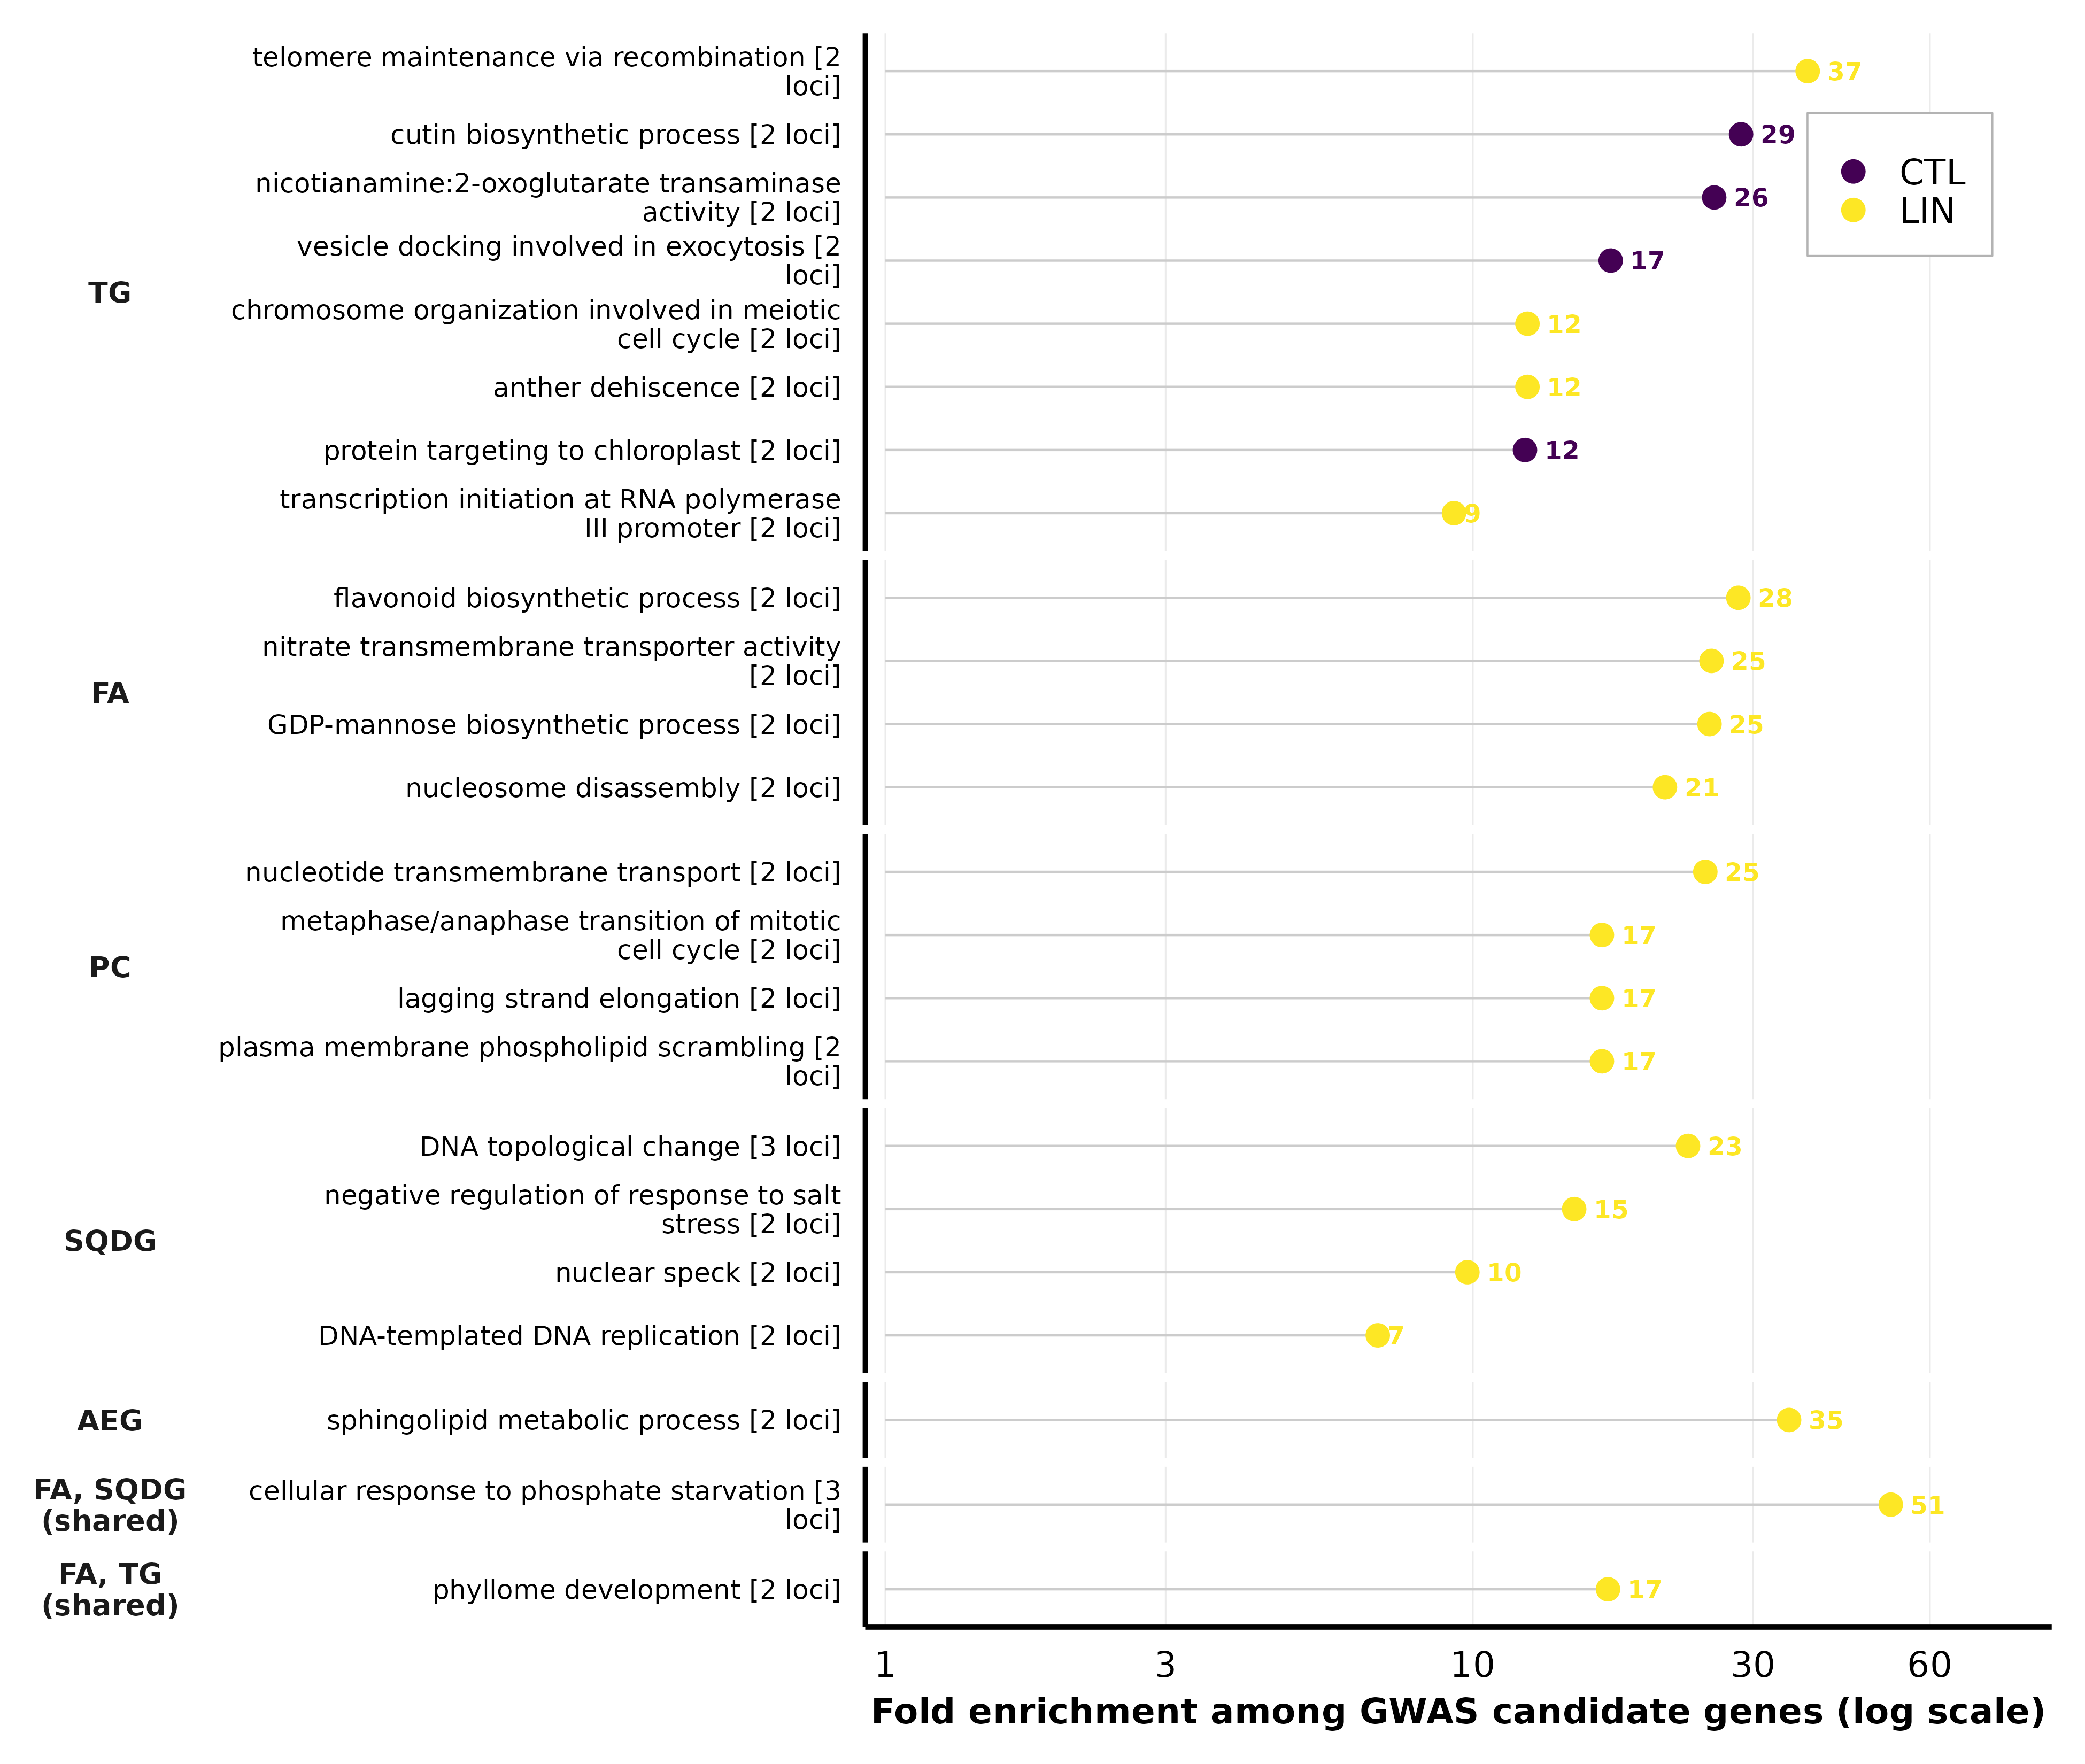
\includegraphics[width=0.95\textwidth]{fig/main/Figure5_GO_BP_LDaware.png}
\caption{Figure 4. GO terms enriched among LD-mapped candidate genes, grouped by
the lipid class whose traits produced them. Nineteen loci shown after collapse
and the 30-background-gene filter.}
\end{figure}

\clearpage
\subsection{Cross-trial overlap collapses to chance at locus level}
\begin{itemize}
  \item \lead{Method.} One-sided hypergeometric (Fisher right-tail) test at two
        resolutions. At \textbf{gene level} the background is the 34{,}027
        annotated \textit{S.~bicolor} v3.1 gene models. At \textbf{locus level}
        the genome is partitioned into non-overlapping 100, 250 and 500~kb
        windows, with background the windows containing at least one annotated
        gene (4{,}844 / 2{,}279 / 1{,}239 respectively). Reported as fold
        enrichment over the expected $|A||B|/N$ plus the Jaccard index, which is
        insensitive to the large size difference between the CTL and LIN sets.
  \item \lead{Gene level looks impressive.} 354 genes shared against 148 expected,
        $2.39\times$, significant in both trait layers.
  \item \lead{It decays to chance once linkage is collapsed.} $1.04\times$ at
        250~kb for individual lipids. Loci recovered in the two trials are no more
        concordant than two independent samples of the same genome.
  \item \lead{Sharing a gene rarely means sharing a phenotype.} Only 25.4\% of the
        354 shared genes were associated with a lipid class in common, falling to
        18.0\% in the individual-lipid layer.
  \item \lead{LD inflates counts three- to five-fold.} CTL 1{,}100 genes
        $\rightarrow$ 378 loci; LIN 4{,}323 $\rightarrow$ 971.
  \item \lead{Class composites are the exception.} They retain a significant
        cross-trial excess at 100 and 250~kb where individual species do not,
        because aggregation averages over acyl-chain heterogeneity and
        measurement noise.
  \item \lead{Take-home.} Cross-environment comparisons must be made at the locus
        level, not the gene level.
\end{itemize}

\begin{figure}[H]
\centering
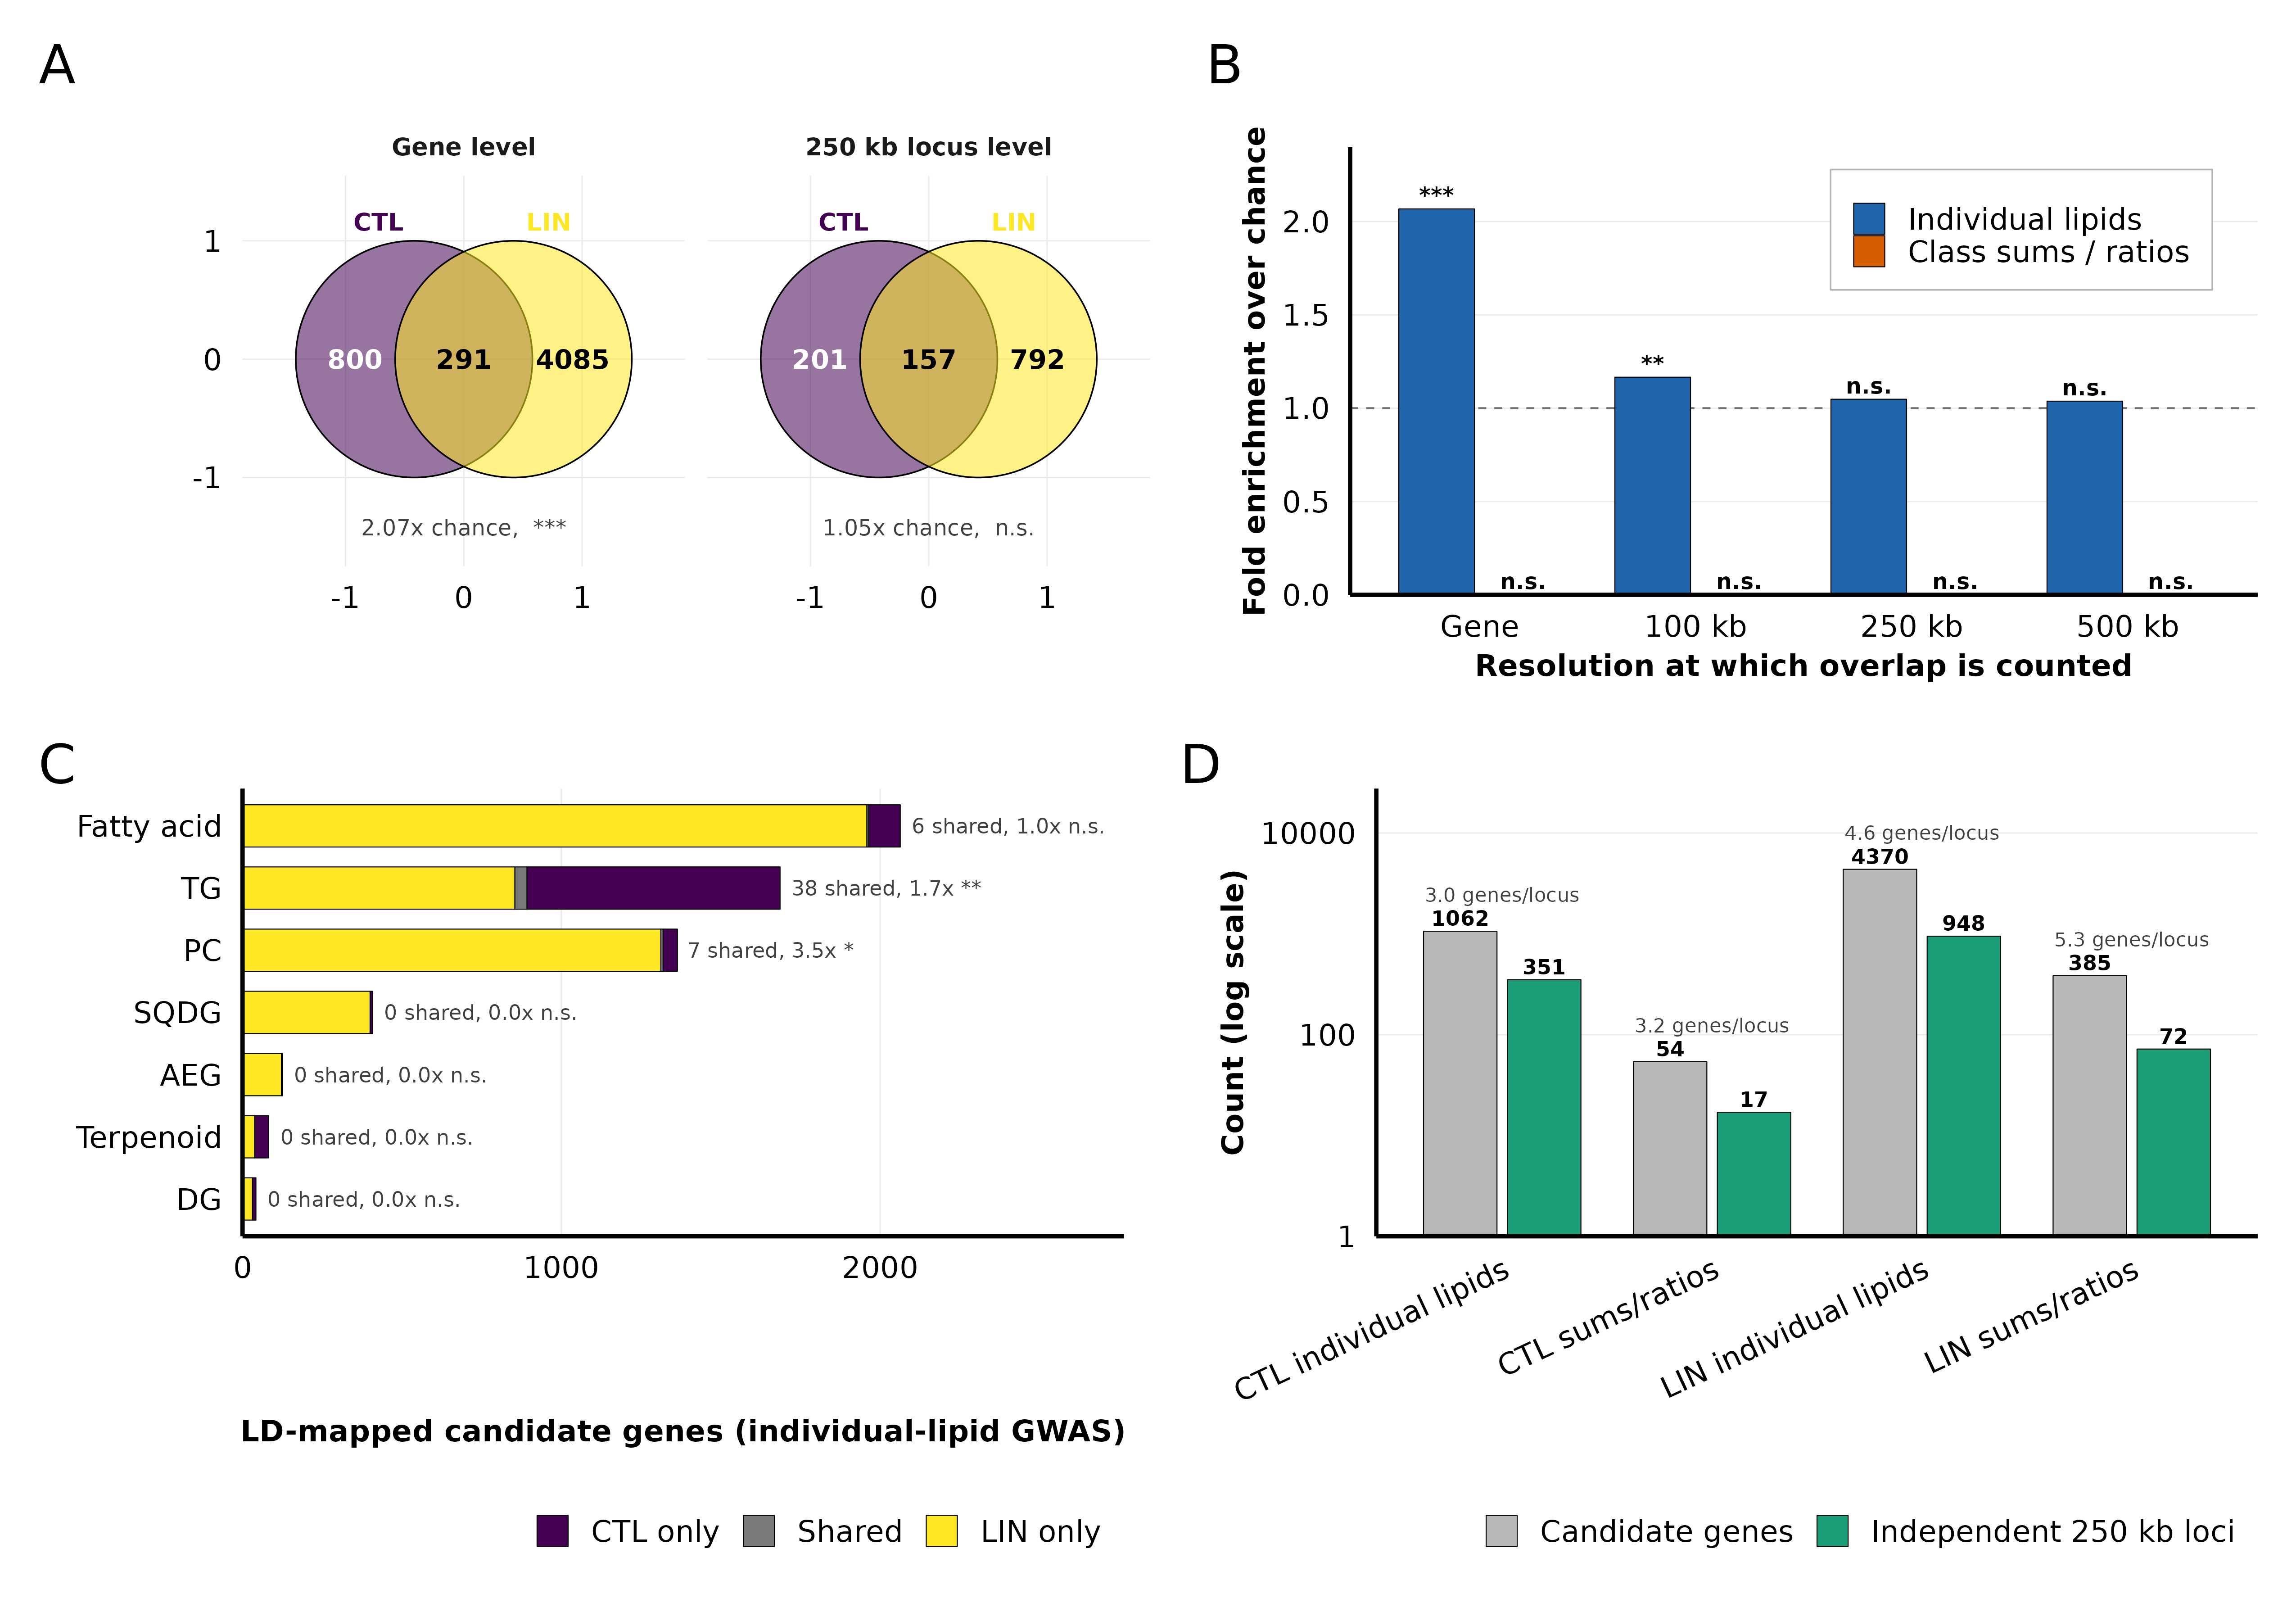
\includegraphics[width=0.82\textwidth]{fig/supp/Figure7_CTL_LIN_Overlap.png}
\caption{Supp.\ Fig.\ S8. Cross-trial candidate overlap at gene and locus
resolution, and its decay with window size.}
\end{figure}

\clearpage
\subsection{LINEX reaction mapping and reaction-balance scoring}
\begin{itemize}
  \item \lead{Method.} LINEX2 reconstructs annotation-guided lipid reaction
        networks from curated rules (head-group interconversion,
        acylation/deacylation, elongation, desaturation). Sorghum is not a
        supported organism, so \textit{Oryza sativa} was the reference -- these
        are therefore hypotheses, not demonstrated flux. Four branches connecting
        the DG/MG, TG and lysophospholipid pools; three from LINEX2, the fourth
        (LCAT*) defined manually from reaction specificity and marked with an
        asterisk throughout.
  \item \lead{Reaction-balance score.} Within one sample,
        $S_i = \mathrm{mean}(\ell_{\mathrm{products}}) -
        \mathrm{mean}(\ell_{\mathrm{substrates}})$, where
        $\ell_{i,c}=\log_{10}(C_{i,c}+\varepsilon_i)$ on class sums.
        Being a within-sample log-ratio, a uniform multiplicative
        difference between the trials cancels -- exactly so in the absence of the
        pseudocount, and to a very good approximation with it. What it does
        \emph{not} remove is an effect acting differentially on lipid classes,
        because a branch's products and substrates are different classes.
        Compared with paired, genotype-matched Wilcoxon tests across the 355
        shared genotypes, which controls for genotype but not for year, planting
        date or acquisition batch. The direction is therefore a description of
        the two trials, not evidence that management caused it.
  \item \lead{Found.} All four branches shift strongly and consistently --
        positive for the three TG-producing branches (PNPLA3 $+0.327$,
        LCAT* $+0.238$, LRO1 $+0.232$) and negative for the hydrolytic
        TG$\rightarrow$DG branch (PNPLA1 $-0.268$), BH-adjusted
        $p<10^{-56}$ across 355 genotype pairs. This recapitulates the
        lipidome-wide picture at the level of a small set of candidate reactions
        rather than as independent class shifts.
\end{itemize}

\begin{figure}[H]
\centering
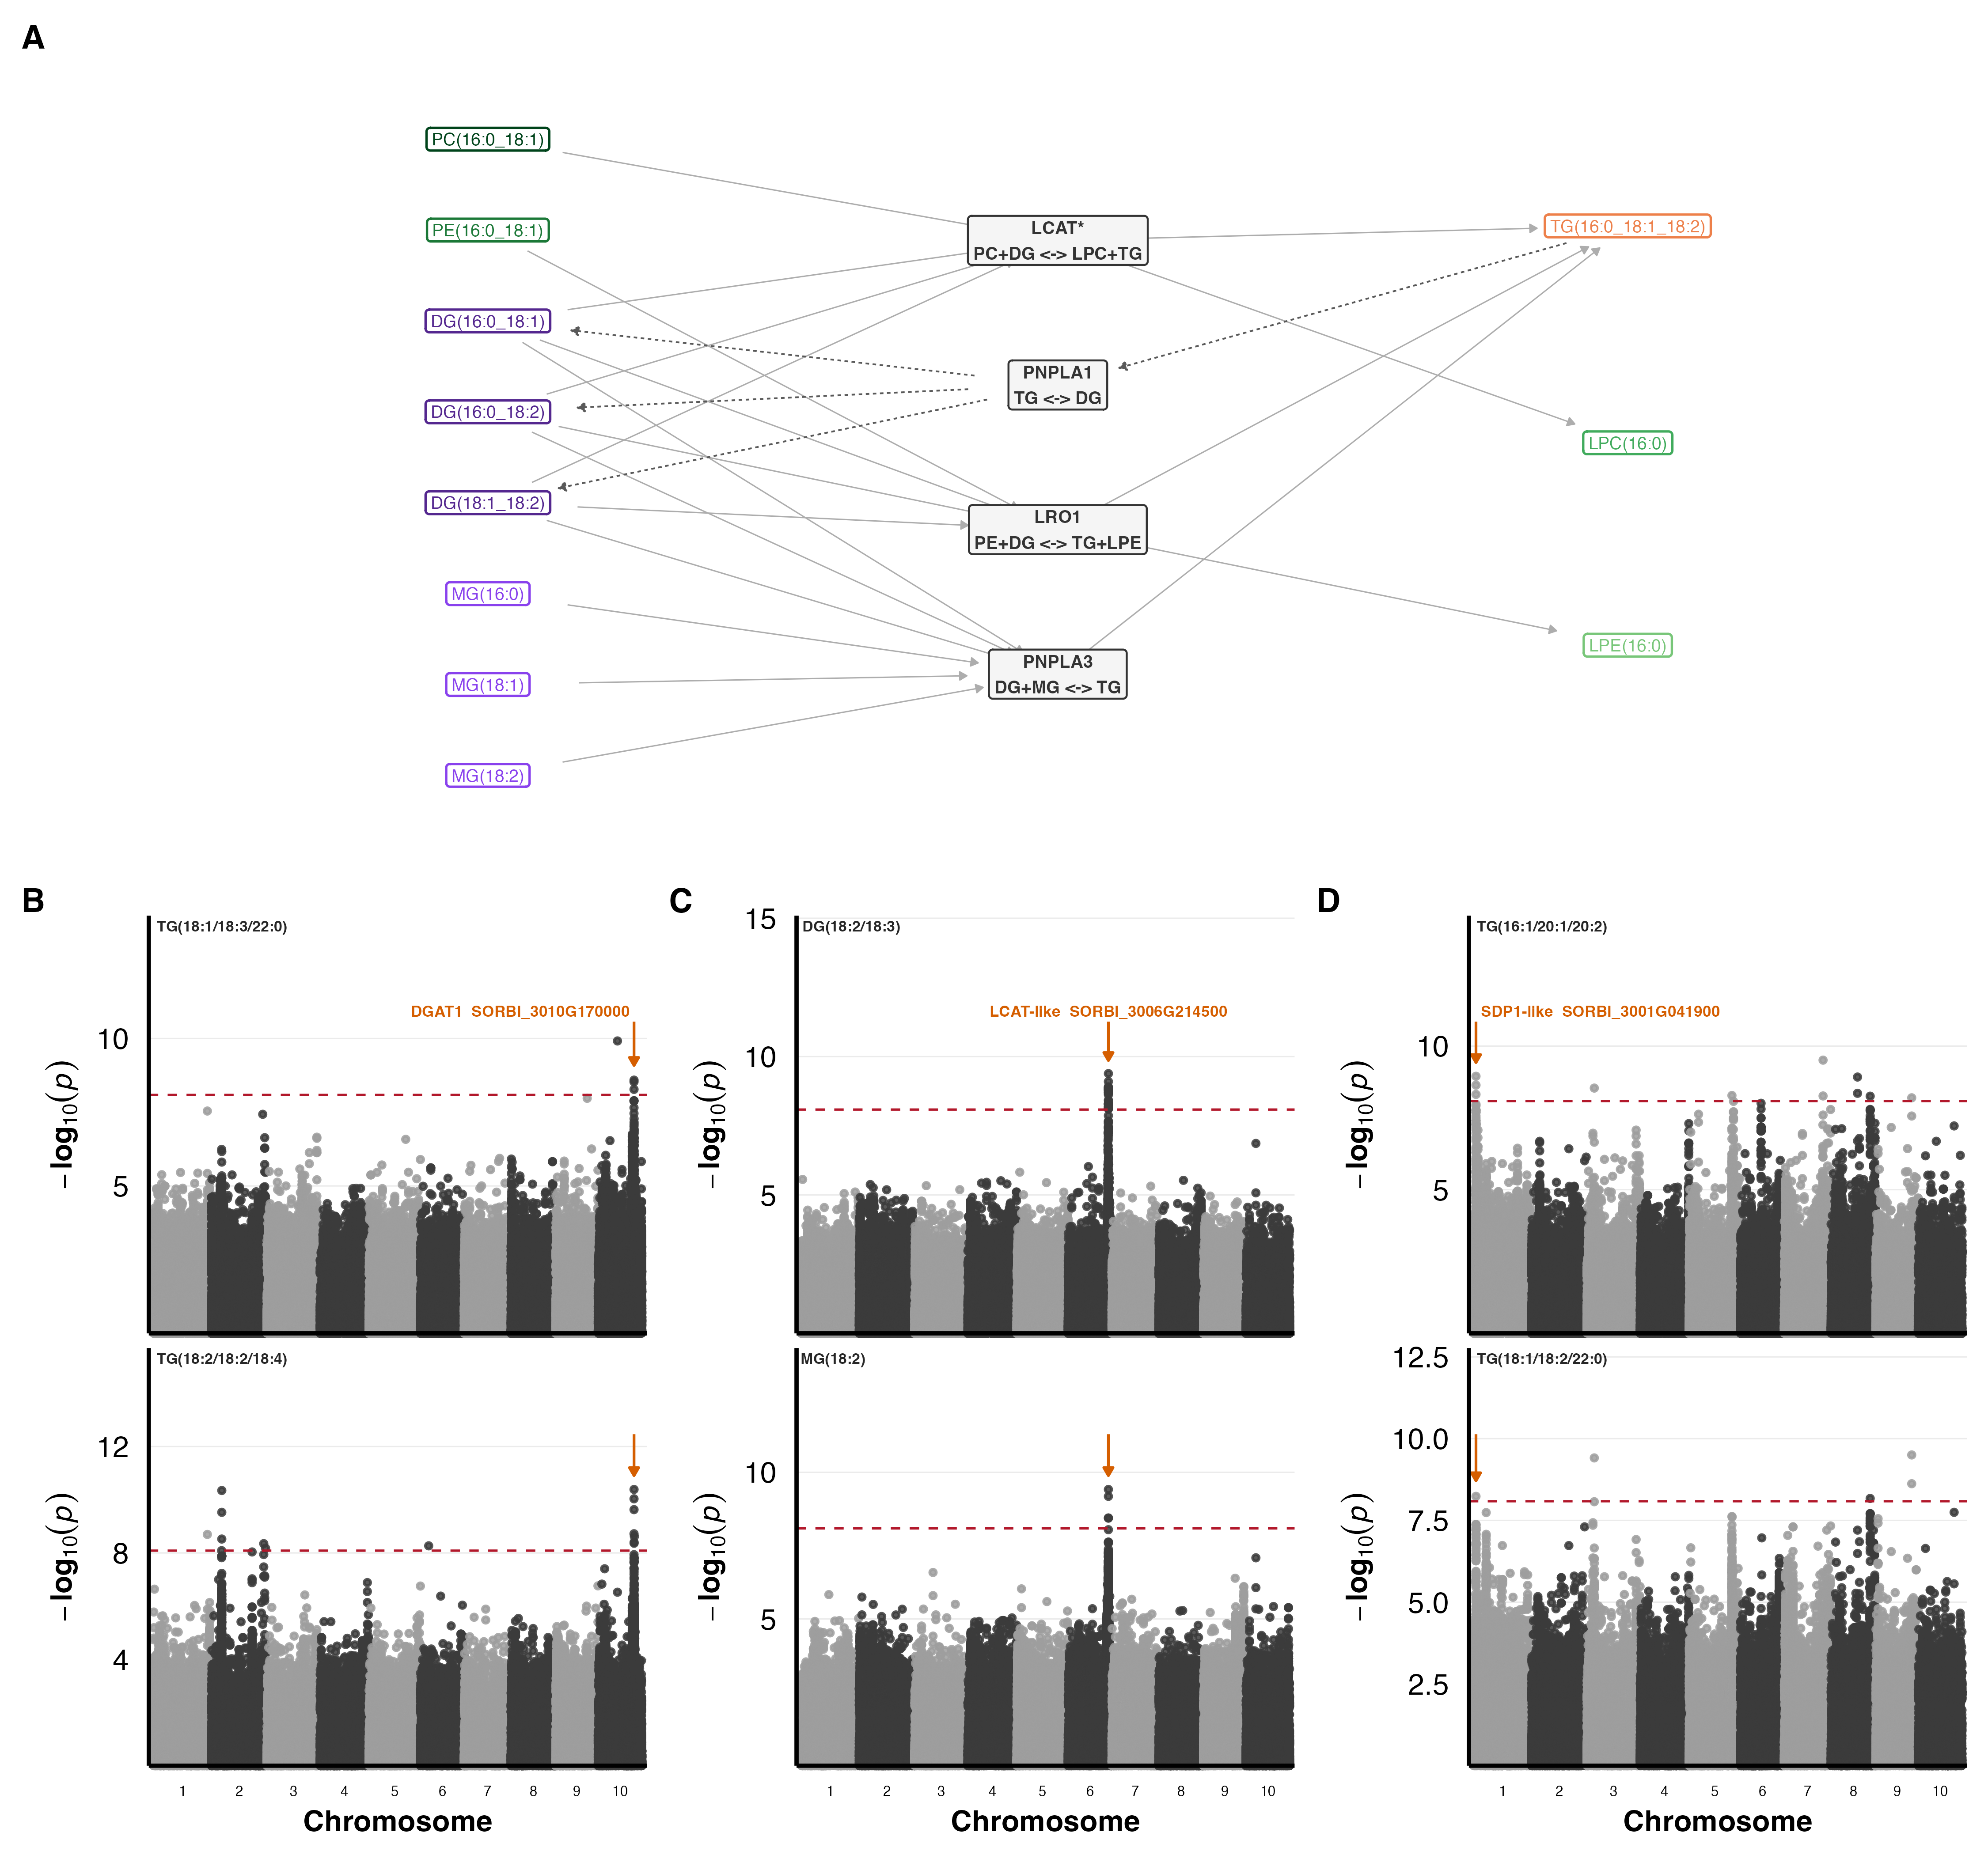
\includegraphics[width=0.95\textwidth]{fig/main/Figure5_LINEX.png}
\caption{Figure 5. LINEX reaction network, branch-level reaction balances, and
GWAS support for the branch-supporting candidate genes.}
\end{figure}

\clearpage
\subsection{Interactive SoLD application}
\begin{itemize}
  \item Fourteen modules -- data preview, boxplots, correlation, PCA,
        t-SNE/UMAP, heatmap, GWAS, gene hits, genotype, Venn, volcano and
        network -- each with dataset and data-type (raw, \%TIC, CLR) selectors.
  \item Worked example moves from a terpenoid class view to lupeol to a terpene
        cyclase annotated for triterpenoid biosynthesis and localised to the lipid
        droplet, demonstrating that classes outside the 13 focal ones remain
        reachable.
\end{itemize}

\begin{figure}[H]
\centering
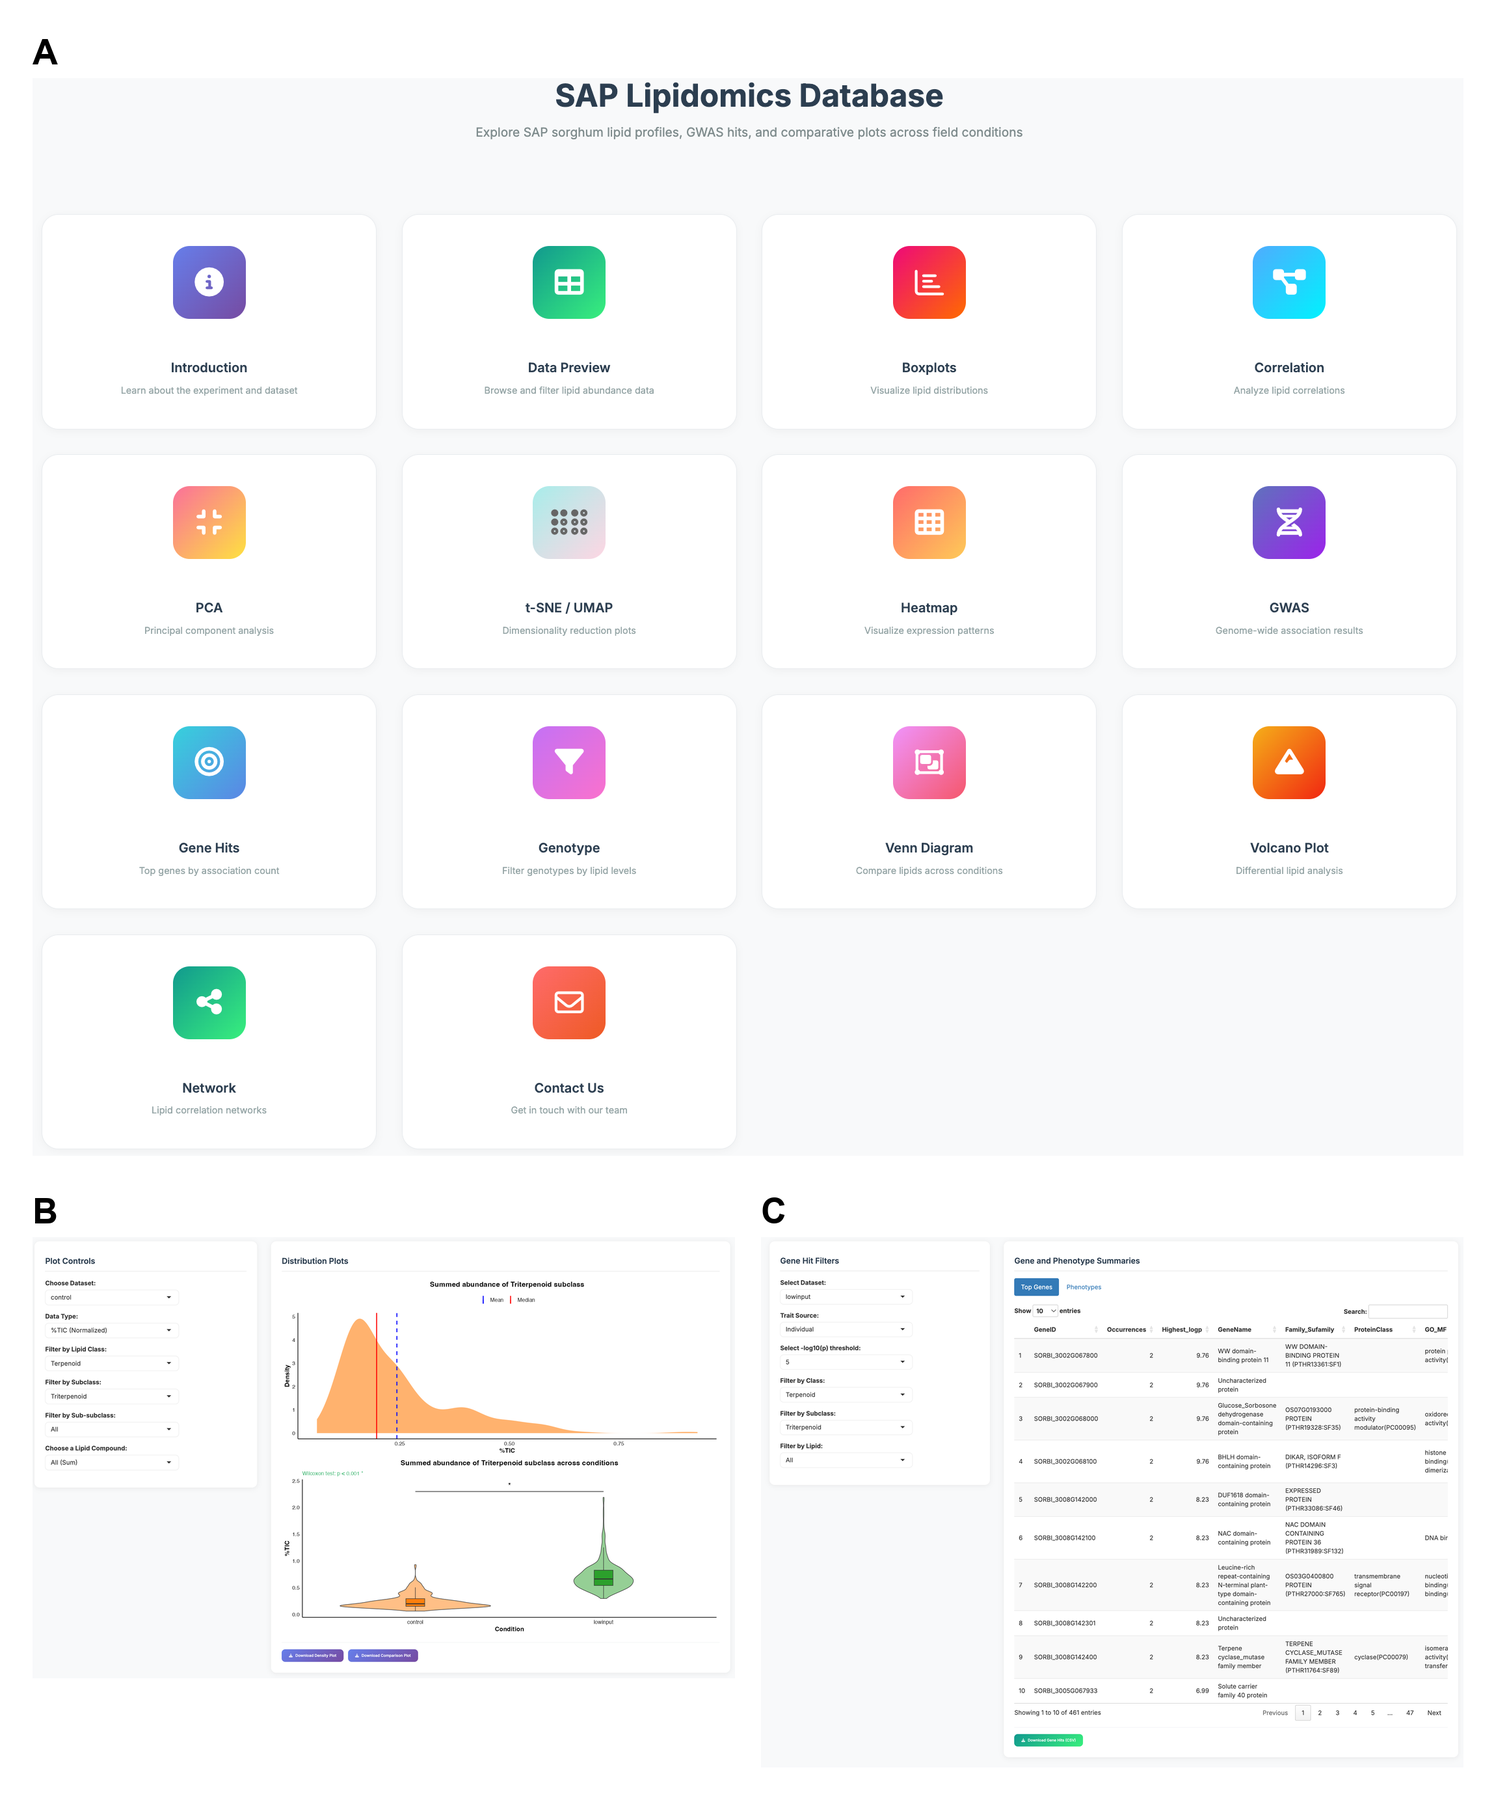
\includegraphics[width=0.9\textwidth]{fig/main/Figure5_shiny_triterpenoid_AB.png}
\caption{Figure 6. The SoLD Shiny application, showing the class-level boxplot
view and the gene-hit table for the same phenotype.}
\end{figure}

\clearpage
\section{Discussion}

\noindent\textbf{Two caveats framing everything below.} Gene functions are
assigned by orthology to characterised genes in other species, so they say what
the family can do, not what the sorghum locus does in a field. And because
candidates come from LD blocks, most regions hold several genes -- an enrichment
resting on fewer than three independent 250~kb intervals is one locus, not a
pathway.

\subsection{Integrated interpretation across the two trials}

\subsubsection*{Why the SQDG decline is the most informative result}
\begin{itemize}
  \item \lead{The expectation it violates.} Under phosphate limitation plants
        replace phospholipids with non-phosphorus surrogates, so SQDG and DGDG
        should \emph{rise}. LIN had reduced P, and SQDG \emph{fell}. Either the
        plants were not experiencing phosphate starvation in the physiological
        sense, or something else overrode the replacement response.
  \item \lead{The phosphate machinery was genetically active.}
        \texttt{SORBI\_3001G028500}, an SPX-domain phosphate-status signalling
        protein of the OsSPX4 type, is a LIN candidate enriched under
        \textit{cellular response to phosphate starvation}, and it associates with
        FA/SQDG and SQDG/FA \emph{ratios} -- i.e.\ with the sulfolipid pool
        specifically. So phosphate status is being sensed and it is genetically
        linked to SQDG; the pool just moves the wrong way.
  \item \lead{Hypothesis 1 -- sulfur, not phosphorus, is the limiting input.}
        SQDG is a plastid lipid whose sulfoquinovose head group is built from
        sulfate imported into the chloroplast and reduced there.
        \texttt{SORBI\_3006G244000} is a SULTR3-family sulfate transporter; in
        Arabidopsis SULTR3 proteins sit in the chloroplast envelope and carry
        plastid sulfate uptake. LIN received no fertiliser and no pesticide, so
        sulfate supply was not topped up either. If plastidic sulfate is short,
        the plant cannot execute the phospholipid-to-sulfolipid swap even while
        sensing low P -- the substrate for the head group is missing. This is the
        cleanest explanation the data support, and it is testable.
  \item \lead{Hypothesis 2 -- the sulfolipid synthases themselves.} Two SQD2-like
        sulfoquinovosyltransferase loci are LIN candidates
        (\texttt{SORBI\_3003G076900}, \texttt{SORBI\_3002G000600}), the enzyme
        that transfers sulfoquinovose onto DAG. Both were recovered through
        fatty-acid phenotypes rather than SQDG levels, so this is suggestive
        rather than established, but it puts allelic variation at the committed
        step of sulfolipid synthesis inside the LIN candidate set.
  \item \lead{Hypothesis 3 -- less thylakoid to put it in.} SQDG is a thylakoid
        membrane lipid. LIN was planted early to impose cold, and cold plus low N
        both reduce photosynthetic membrane per unit tissue. A smaller plastid
        membrane compartment lowers SQDG regardless of phosphate status. MGDG and
        DGDG behaviour is consistent with a plastid-membrane component to the
        shift.
  \item \lead{Hypothesis 4 -- severity and stage.} Classical replacement is
        described under severe or complete P withdrawal, usually hydroponic. LIN
        was \emph{reduced} P in field soil with a residual pool, and sampled at a
        single developmental stage that differed from CTL. A partial P deficit may
        simply never cross the threshold that triggers membrane lipid replacement.
  \item \lead{The phosphate transporter points the same way.}
        \texttt{SORBI\_3002G116100}, a PHT1-family H$^{+}$/Pi cotransporter whose
        closest characterised rice relative is OsPT4, is a LIN candidate for five
        species at $p=1.1\times10^{-9}$ ($r^2=0.87$) -- and four of the five are
        \emph{neutral storage lipids}, including TG(18:3\_18:3\_18:3), not
        phospholipids. A phosphate transporter reporting on triacylglycerol is
        the opposite of what phospholipid-to-glycolipid replacement predicts. It
        is the weakest association discussed and only marginally clears
        Bonferroni, so it is a pointer, not a pillar.
  \item \lead{What we can and cannot claim.} We can say the LIN lipidome is not
        the textbook phosphate-starvation lipidome, and that the candidate genes
        put sulfur supply and sulfolipid synthesis on the table as the
        alternative. We cannot attribute the decline to any single factor,
        because nutrient level, temperature, planting date, developmental stage
        and year are confounded in this design.
\end{itemize}

\subsubsection*{The rest of the integrated picture}
\begin{itemize}
  \item TG accumulation comes with reorganised DG--TG coordination rather than a
        uniform rise in neutral lipids -- ratios involving TG, DG, PE and MGDG all
        shift toward TG, the PS--TG correlation changes sign, and the LINEX
        balances split by branch direction (three TG-producing branches positive,
        the hydrolytic TG$\rightarrow$DG branch negative).
  \item PS rose relative to other phospholipids and its correlation with PC
        reversed, which is head-group redistribution inside a reorganised network
        rather than membrane expansion. PE gained the most unsaturation of any
        membrane class. But PS and the lysophospholipids are each under 0.2\% of
        TIC against tens of percent for MGDG, so these are redistributions within
        small pools, and compositional transforms exaggerate them. PS is also the
        only trait clearly structured by genetic cluster, and only under LIN.
  \item Genetic architecture is strongly environment-dependent -- after collapsing
        linkage blocks, CTL and LIN loci overlap no more than chance
        ($1.04\times$ at 250~kb) and only ${\sim}25\%$ of shared genes map to the
        same lipid class. Class-level composites are the exception and are the
        more robust unit for cross-environment comparison. Genotype-by-nutrient
        cannot be separated from genotype-by-year or genotype-by-management here.
\end{itemize}

\subsection{A TIFY/JAZ cluster recovered in both trials}
\begin{itemize}
  \item Four TIFY paralogues in a 290~kb stretch on chromosome~1 --
        \texttt{SORBI\_3001G259300}, \texttt{SORBI\_3001G259400} and
        \texttt{SORBI\_3001G259600} -- \lead{recovered under both regimes but
        reporting different lipids}. Under CTL, \texttt{SORBI\_3001G259400} and
        \texttt{SORBI\_3001G259600} associate with nine 16:0-containing storage
        triacylglycerols, e.g.\ TG(16:0\_18:1\_18:1) and TG(16:0\_18:1\_20:1).
        Under LIN those two plus \texttt{SORBI\_3001G259300} instead associate
        with AEG(o-15:2\_15:0), PC(14:0\_18:3) and 11,14,17-eicosatrienoic acid,
        with the top signal strengthening to $p=1.6\times10^{-12}$.
  \item \lead{Mechanistically tight rather than coincidental.} JAZ/TIFY proteins
        are the repressors of jasmonate signalling, and jasmonate is made from
        $\alpha$-linolenic acid (18:3) released from plastid galactolipids. The
        LIN traits carry exactly that chemistry -- an 18:3 phosphatidylcholine and
        a free C20:3 fatty acid.
  \item In the AEG test the cluster maps to a collapsed locus for
        \textit{regulation of defense response}, \textit{regulation of jasmonic
        acid mediated signaling pathway} and \textit{response to wounding},
        enriched 34.5-fold over sixteen background genes
        ($q_{\mathrm{LD}}=0.0068$) -- and unlike the other tandem loci, on
        \emph{two} independent 250~kb intervals, not one.
  \item Cold support in three systems -- rice \textit{OsTIFY} (cold-induced,
        ABA-independent), pepper \textit{CaTIFY7}/\textit{CaTIFY10b} (silencing
        confers cold sensitivity, overexpression improves tolerance) and
        coordinated cold induction in sweet orange. LIN was planted early to
        impose cold, so this fits.
  \item \lead{Caveats.} LD peaks at $r^2=0.88$, so the causal variant could be any
        of the four paralogues or a neighbour; trial-specific associations do not
        prove functional switching, since only genome-wide-significant traits are
        counted; and three genes against sixteen background makes the fold
        estimate imprecise.
\end{itemize}

\subsection{Under CTL, membrane organization and amino-acid metabolism}
\begin{itemize}
  \item \lead{The membrane link.} \texttt{SORBI\_3006G040500}, a
        phospholipid-transporting P4-type ATPase, associated with 27 TG
        phenotypes. P4-ATPases are flippases that move lipids between membrane
        leaflets; the Arabidopsis relative ALA2 is strongly PS-specific. It
        contributes to no enriched term and is carried on annotation alone.
  \item \lead{The tyrosine locus is the more interesting half.} The enriched term
        is \textit{L-tyrosine catabolic process}, four genes on three chromosomes,
        and \emph{every} phenotype at those loci is a triacylglycerol. Tyrosine
        degradation runs through tyrosine aminotransferase and 4-hydroxyphenyl\-%
        pyruvate dioxygenase to homogentisate, then to fumarate and
        \lead{acetoacetate, which feeds acetyl-CoA} -- the substrate for
        fatty-acid synthesis.
  \item \texttt{SORBI\_3005G152200}, a chromosome~5 aminotransferase, alone
        explains the nine-species 16:0 TAG block ($p=9.7\times10^{-13}$).
        \texttt{SORBI\_3002G104200}, annotated with HPPD activity, places the next
        step of the same pathway at an unlinked locus.
  \item \lead{The same amino acid is committed to dhurrin under LIN}, so tyrosine
        is a single metabolic branch point that the two trials resolve
        differently -- catabolism to lipid carbon under CTL, cyanogenic glucoside
        synthesis under LIN.
  \item \lead{Caveat.} Two adjacent chromosome~2 genes fall in the nicotianamine
        aminotransferase subfamily (iron-uptake phytosiderophores in grasses), and
        the same three genes are enriched for both the tyrosine transaminase and
        the nicotianamine transaminase terms -- annotation ambiguity within one
        subfamily. $\alpha$-Tocopherol, the other homogentisate route, maps 1.1~Mb
        away, so the two are separable here.
\end{itemize}

\subsection{Under LIN, nitrogen candidates}
\begin{itemize}
  \item \lead{Uptake.} Three nitrate transporters from two families --
        \texttt{SORBI\_3004G009400} (NRT2.1-like, high-affinity; drives nitrate
        transport/assimilation enrichment in both the FA and SQDG sets),
        \texttt{SORBI\_3008G081400} (NPF/NRT1; the strongest LIN single-lipid
        association in the panel) and \texttt{SORBI\_3001G133900}, whose rice
        orthologue OsNPF2.4 handles low-affinity root-to-shoot nitrate transfer.
  \item \lead{Storage rather than uptake.} A chromosome~1 locus overlapping the
        dhurrin cluster links seven candidates to FA(22:1),
        11,14,17-eicosatrienoic acid, TG(14:0\_18:3\_18:3) and twelve of the
        thirteen PA-to-class ratios. Four of the seven cover consecutive steps of
        dhurrin metabolism -- a CYP71E1-reaction monooxygenase
        (\texttt{SORBI\_3001G012000}, $r^2=1.00$), a glycosyltransferase
        (\texttt{SORBI\_3001G012400}), a MATE-family vacuolar transporter
        (\texttt{SORBI\_3001G012600}, $r^2=1.00$) and a glutathione transferase
        (\texttt{SORBI\_3001G012500}).
  \item \lead{The logic.} Nitrogen induces dhurrin synthesis in older sorghum, so
        under reduced N less tyrosine-derived carbon and nitrogen is committed to
        dhurrin, freeing precursor for lipid synthesis. Consistent with the
        associations being \emph{ratios} rather than individual species. Dhurrin
        itself was not measured, so this rests on annotation inside one LD block.
\end{itemize}

\subsection{Under LIN, phosphorus and sulfur converge on SQDG}
\begin{itemize}
  \item The three genes are \texttt{SORBI\_3001G028500} (SPX phosphate-status
        signalling), \texttt{SORBI\_3006G244000} (SULTR3 plastid sulfate
        transporter) and \texttt{SORBI\_3002G116100} (PHT1 phosphate
        transporter) -- see the SQDG discussion above, where each is used.
  \item \lead{The one-line argument.} Phosphate limitation alone should
        \emph{increase} SQDG; SQDG was depleted; a sulfolipid needs sulfur, and a
        plastid sulfate transporter is sitting in the candidate set. Restricted
        plastidic sulfate supply is the plausible alternative hypothesis, not a
        demonstrated mechanism.
\end{itemize}

\subsection{Under LIN, a cold-induced MADS regulator}
\begin{itemize}
  \item \texttt{SORBI\_3003G406800}, a MADS-box transcription factor and the
        \lead{strongest LIN fatty-acid association in the panel}
        ($p=2.7\times10^{-17}$), lead SNP intragenic ($r^2=1$), signal recurring
        across FA(22:1), PC(18:2\_20:4), total FA and multiple FA-to-class ratios.
  \item Cold-induced in sorghum within 6~h (log$_2$FC 1.04, adj.\
        $p=5.7\times10^{-19}$) and a hub of the early shock-phase co-expression
        module ($k_{\mathrm{ME}}=0.91$).
  \item Its closest annotated maize homologue at 84\% identity is
        \textit{ZmMADS69}, the flowering-time QTL acting through ZmRap2.7 to
        relieve repression of the florigen \textit{ZCN8}, and a target of
        tropical-to-temperate selection.
  \item LIN was planted early specifically to impose cold, and cold acclimation
        proceeds partly through acyl-chain remodelling, which makes fatty-acid
        traits the expected point of contact. The association may reflect direct
        regulation of lipid metabolism or a shift in developmental stage at
        sampling; this design cannot separate them.
\end{itemize}

\subsection{Reaction-supported remodeling candidates under LIN}
\begin{itemize}
  \item \lead{DG input.} \texttt{SORBI\_3003G107900}, non-specific phospholipase~C6,
        associates with PC(18:2\_20:4), a plausible substrate --
        \lead{but linkage cannot separate it from five sterol C-8 isomerase
        (EXPERA) genes in the same 137~kb window on chromosome~3}. All six share
        one association with the same species at $r^2\ge0.95$ and together form
        the most specifically annotated locus in the enrichment set (13.6-fold
        over six background genes).
  \item \lead{Branch (i), PC$+$DG$\leftrightarrow$LPC$+$TG.} Two LCAT-superfamily
        candidates -- \texttt{SORBI\_3006G214500}, which links to the branch
        substrates DG(18:2\_18:3) and MG(18:2), and
        \texttt{SORBI\_3004G341900}, annotated as a phospholipid--sterol
        O-acyltransferase. The second allows an alternative chemistry: sterol
        esterification using PC as acyl donor would release LPC \emph{without}
        producing TG. That fits LIN sterol demand, where $\beta$-sitosterol rises
        more than four-fold -- the largest proportional superclass change -- and
        it dovetails with the EXPERA cluster above.
  \item \lead{TG synthesis.} \textit{DGAT1} (\texttt{SORBI\_3010G170000}) is the
        clearest genetic link to the TG phenotype, sitting under a repeatedly
        mapped chromosome~10 crude-fat QTL, with five of six associated phenotypes
        polyunsaturated triacylglycerols including TG(18:3\_18:3\_18:3).
  \item \lead{TG breakdown.} \texttt{SORBI\_3001G041900}, an \textit{SDP1}-like
        patatin lipase clustering with \textit{SbSDP1-L}, associates with three TG
        species and, at class level, with total TG and the TG/SQDG ratios --
        a bulk-pool lipase rather than a species-specific one.
  \item \lead{A sphingolipid module outside the DG--TG branches.} Three genes
        spanning three consecutive pathway steps on three chromosomes -- a serine
        C-palmitoyltransferase (\texttt{SORBI\_3001G434900}), a DAGK-domain kinase
        (\texttt{SORBI\_3007G041500}) and a ceramide glucosyltransferase
        (\texttt{SORBI\_3003G394100}) -- all associated with AEG(o-15:2\_15:0),
        the only ether-linked species that increases under LIN. Supported by
        three independent intervals. This is genetic evidence, not abundance
        evidence: sphingolipid levels barely change and the species are trace.
        Still the most complete candidate pathway in the study and the most
        direct target for functional follow-up.
\end{itemize}
\vspace{8pt}
\hrule
\vspace{6pt}

\noindent\textbf{What is novel methodologically.} The LD-aware permutation null
and the two-pass gene-set collapse for GO enrichment, and the demonstration that
gene-level GWAS overlap between environments is largely a linkage artefact that
disappears at locus level.

\end{document}
